\documentclass{report}

\usepackage{amsmath, array, bm, enumerate, tikz, pgfplots, sfmath, multicol, hyperref, afterpage, cclicenses}
\pgfplotsset{compat = newest}
\usepackage[margin = 0.5in]{geometry}
\raggedright
\renewcommand{\familydefault}{\sfdefault}
\newcounter{Review}
\usetikzlibrary{fadings}

\begin{document}

\newcommand\bigangle[2][]{% 
    \draw[->,domain=0:#2,variable=\t,samples=200,>=stealth,#1]
      plot ({(\t+#2)*cos(\t)/(4*#2)},
           {(\t+#2)*sin(\t)/(4*#2)}) 
        ;}

\begin{titlepage}
\DeclareFixedFont{\titlefont}{T1}{ppl}{b}{}{0.7in}
\DeclareFixedFont{\subtitlefont}{T1}{ppl}{b}{}{0.4in}
\afterpage{\restoregeometry}
\newgeometry{left=1in, right=1in,top=1in, bottom=0in}
\definecolor{stainedglassblue}{HTML}{2E37FE}
\pagecolor{stainedglassblue}\afterpage{\nopagecolor}

\thispagestyle{empty}
\begin{center}
\color{white}{
\titlefont Honors PreCalculus	\vfill
%\scalebox{3}{${\displaystyle \sum_{\text{Algebra}}^{\text{Trigonometry}}  } $}
%\vfill 
\subtitlefont Extra Practice}
\end{center}
\vfill
\end{titlepage}


\tableofcontents
\chapter{Basic Set Theory and Interval Notation}

You are given either interval notation, set-builder notation, or a graph. Write each of the following in its other 2 forms. 
\begin{enumerate}
\setlength\itemsep{10pt}
    \item $(-5, 8]$
    \item $\{x|x \leq 1\}$
    \item
    \raisebox{-8pt}{
    \begin{tikzpicture}
    \draw [->] (-2,0) node [below, yshift=-4pt] {$-3$} -- (2,0);
    \draw [fill=black] (-2,0) circle [radius=2.5pt];
    \end{tikzpicture}}
    \item $\{x | x \neq 4, 11\}$
    \item
    \raisebox{-8pt}{
    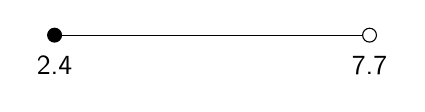
\begin{tikzpicture}
        \draw (-2,0) node [below, yshift=-4pt] {$2.4$} -- (2,0) node [below, yshift=-4pt] {$7.7$};
        \draw [fill=black] (-2,0) circle [radius=2.5pt];
        \draw [fill=white] (2,0) circle [radius=2.5pt];
    \end{tikzpicture}}
    \item $(9, \infty)$
\setcounter{Review}{\value{enumi}}
\end{enumerate}

Write each using interval notation and graph on a number line.
\begin{enumerate}
\setcounter{enumi}{\value{Review}}
\item $\{x | x \geq 2\}$
\item $\{x |x < -8\}$
\item $\{x |x \neq 3\}$
\item $\{x | x \neq -2, 5\}$
\setcounter{Review}{\value{enumi}}
\end{enumerate}

You are given the graph of an interval. Write the interval and set-builder notation for it.
\begin{enumerate}
\setcounter{enumi}{\value{Review}}
\item \raisebox{-10pt}{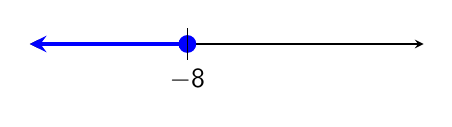
\begin{tikzpicture}[>=stealth]
    \draw[<->] (-2.5,0) -- (2.5,0);
    \filldraw[color=blue] (-0.5,0) circle [radius=3pt];
    \draw (-0.5,0.2) -- (-0.5,-0.2) node [below] {$-8$};
    \draw[color=blue,ultra thick, ->] (-0.5,0) -- (-2.5,0);
    \end{tikzpicture}}

\item \raisebox{-10pt}{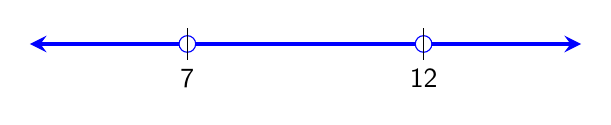
\begin{tikzpicture}[>=stealth]
    \draw[<->, color=blue, ultra thick] (-3.5,0) -- (3.5,0);
    \draw[color=blue, fill=white] (-1.5,0) circle [radius=3pt];
    \draw[color=blue, fill=white] (1.5,0) circle [radius=3pt];
    \draw (-1.5,0.2) -- (-1.5,-0.2) node [below] {$7$};
    \draw (1.5,0.2) -- (1.5,-0.2) node [below] {$12$};
    \end{tikzpicture}}
\end{enumerate}

\newpage

\textsc{Basic Set Theory and Interval Notation Key}

\begin{enumerate}
\setlength\itemsep{10pt}
	\item $\{x | -5 < x \leq 8\}$	\newline\\
	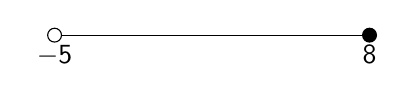
\begin{tikzpicture}
	\draw (-2,0) node [below] {$-5$} -- (2,0) node [below] {$8$};
	\draw [fill=white] (-2,0) circle [radius = 2.5pt];
	\draw [fill=black] (2,0) circle [radius = 2.5pt];
	\end{tikzpicture}
	
	\item $(-\infty, 1]$ \newline\\
	\begin{tikzpicture}
	\draw [<-] (-2,0) -- (2,0) node [below] {1};
	\draw [fill=black] (2,0) circle [radius=2.5pt];
	\end{tikzpicture}
	
	\item $[-3, \infty)$ \quad $\{x | x \geq -3 \}$
	
	\item $(-\infty, 4) \cup (4, 11) \cup (11, \infty)$ \newline\\
	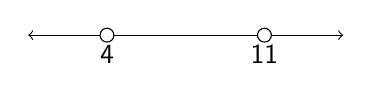
\begin{tikzpicture}
	\draw[<->] (-2,0) -- (2,0);
	\draw[fill=white] (-1,0) circle [radius=2.5pt];
	\draw[fill=white] (1,0) circle [radius=2.5pt];
	\node at (-1,0) [below] {4};
	\node at (1,0) [below] {11};
	\end{tikzpicture}
	
	\item $[2.4, 7.7)$ \quad $\{x | 2.4 \leq x < 7.7\}$
	
	\item $\{x | x > 9\}$ \newline\\
	\begin{tikzpicture}
	\draw[->] (-2,0) -- (2,0);
	\draw[fill=white] (-2,0) circle [radius=2.5pt];
	\node at (-2,0) [below] {9};
	\end{tikzpicture}

	\item $[2, \infty)$ \newline\\
	\begin{tikzpicture}
	\draw[->] (-2,0) -- (2,0);
	\draw[fill=black] (-2,0) circle [radius=2.5pt];
	\node at (-2,0) [below] {2};
	\end{tikzpicture}
	
	\item $(-\infty, -8)$ \newline\\
	\begin{tikzpicture}
	\draw[<-] (-2,0) -- (2,0);
	\draw[fill=white] (2,0) circle [radius=2.5pt];
	\node at (2,0) [below] {$-8$};
	\end{tikzpicture}
	
	\item $(-\infty, 3) \cup (3, \infty)$ \newline\\
	\begin{tikzpicture}
	\draw[<->] (-2,0) -- (2,0);
	\draw[fill=white] (0,0) circle [radius=2.5pt];
	\node at (0,0) [below] {3};
	\end{tikzpicture}
	
	\item $(\infty, -2) \cup (-2,5) \cup (5,\infty)$ \newline\\
	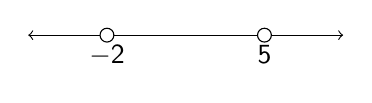
\begin{tikzpicture}
	\draw[<->] (-2,0) -- (2,0);
	\draw[fill=white] (-1,0) circle [radius=2.5pt];
	\draw[fill=white] (1,0) circle [radius=2.5pt];
	\node at (-1,0) [below] {$-2$};
	\node at (1,0) [below] {5};	
	\end{tikzpicture}
	
	\item $(-\infty, -8]$ \quad $\{ x | x \leq -8 \}$
    \item $(-\infty,7) \cup (7,12) \cup (12, \infty)$ \quad $\{ x | x \neq 7, 12 \}$
\end{enumerate}



\chapter{Functions and Their Graphs}

\section{Evaluating Functions}

Given $f(x) = -3x^2 + 4x$ and $g(x) = \frac{1}{x}-5$, evaluate each.
\begin{enumerate}
	\item $f(5)$
	\item $f(-2)$
	\item $f(0)$
	\item $g(1)$
	\item $g(-5)$
	\item $g(1/4)$
\end{enumerate}

\section{Domain of Functions}

Find the domain of each write your answers in interval notation.
\begin{multicols}{2}
\begin{enumerate}
	\item $f(x) = -8x^2 - 7x + 1$
	\item $g(x) = \sqrt{5x+12}-2$
	\item $h(x) = \frac{x+2}{9x-7}$
	\item $f(x) = -5x + 4$
	\item $f(x) = x^2 + 2$
	\item $f(x) = \frac{2x+1}{3x-5}$
	\item $f(x) = \sqrt{3x-12}$
	\item $f(x) = \frac{x}{x^2-16}$
	\item $f(x) = \frac{x+4}{x^3-4x}$
	\item $f(x) = \frac{x}{\sqrt{x-4}}$
	\item $f(x) = \frac{x^2+1}{2x^2+8}$
	\item $f(x) = -\frac{x+7}{x^2-5x-6}$
	\item $g(x) = \sqrt{2x+3}$
	\item $h(x) = \sqrt[3]{2x+3}$
	\item $f(x) = -\frac{7x-10}{x^2+3x+2}$
	\item $g(x) = \sqrt{-9x+8}$
	\item $h(x) = -\sqrt[3]{4x+1}$
	\item $f(x) = \sqrt[3]{8x+1}$
	\item $g(x) = \frac{x^2-1}{\sqrt{x+3}}$
	\item $h(x) = \frac{3}{9 + \frac{4}{x+7}}$
	\item $f(x) = \frac{x+1}{\sqrt{10x+8}}$
	\item $g(x) = \frac{5}{1+\frac{3}{x+2}}$
	\item $i(x) = \frac{7}{3-\frac{4}{x+1}}$
	\item $n(x) = \frac{7x+14}{\sqrt{2x-1}}$
	\item $a(x) = \dfrac{\frac{x}{x-2}}{{\frac{3}{x-2}+6}}$
	\item $d(x) = \frac{7x-5}{\sqrt[3]{5x+2}}$
\end{enumerate}
\end{multicols}

\section{Piecewise Functions}

Find the value of each given the piecewise function below. Use exact answers when possible.
\[
f(x) = \begin{cases}
    x^2-1   &\text{if } x < -3 \\
    0.2x+7  &\text{if } -3 \leq x < 2   \\
    \sqrt{5x}   &\text{if } x \geq 2    \\
\end{cases}
\]
\begin{enumerate}
\item $f(3)$
\item $f(0)$
\item $f(-2)$
\item $f(-3)$
\item $f(0.5)$
\setcounter{Review}{\value{enumi}}
\end{enumerate}

Find each of the following given the piecewise function
\[f(x) = 
\begin{cases}
x^2-7 & x \leq -4 \\
\sqrt{2x+7} & -4 < x < 0 \\
|-x-1| & x \geq 0 \\
\end{cases}
\]
\begin{enumerate}	\setcounter{enumi}{\value{Review}}
\item $f(3)$
\item $f(-2)$
\item $f(0)$
\item $f(-5)$
\setcounter{Review}{\value{enumi}}
\end{enumerate}

Find the value of each given the piecewise function below. Round to 3 decimal places when necessary.

\[
 f(x) = 
 \begin{cases}
    x^2 - 5 \quad &\text{if } x \leq -3 \\[6pt]
    
    \sqrt{-4x + 1} \quad &\text{if } -3 < x \leq 0 \\[6pt]
    
    \frac{5x^2}{x+7} \quad &\text{if } x > 0 \\
 \end{cases}
\]

\begin{enumerate}	\setcounter{enumi}{\value{Review}}
\item $f(7)$
\item $f(-3)$
\item $f(1)$
\item $f(0)$
\item $f(-1)$
\item $f(-3/2)$
\end{enumerate}

\newpage

\textsc{Functions and Their Graphs Key}	

\section*{Evaluating Functions}

\begin{enumerate}
	\item $-55$
	\item $-20$
	\item 0
	\item $-4$
	\item $-5.2$
	\item $-1$
\end{enumerate}

\section*{Domain of Functions}

\begin{multicols}{2}
\begin{enumerate}
	\item $(-\infty, \infty)$
	\item $\left[\frac{-12}{5}, \infty\right)$
	\item $\left(-\infty, \frac{7}{9}\right) \cup \left(\frac{7}{9}, \infty\right)$
	\item $(-\infty, \infty)$
	\item $(-\infty, \infty)$
	\item $\left(-\infty, \frac{5}{3}\right) \cup \left(\frac{5}{3}, \infty\right)$
	\item $[4, \infty)$
	\item $(-\infty, -4) \cup (-4, 4) \cup (4, \infty)$
	\item $(-\infty, -2) \cup (-2, 0) \cup (0,2) \cup (2, \infty)$
	\item $(4, \infty)$
	\item $(-\infty, \infty)$
	\item $(-\infty, -1) \cup (-1, 6) \cup (6, \infty)$
	\item $\left[-\frac{3}{2}, \infty\right)$
	\item $(-\infty, \infty)$
	\item $(-\infty, -2) \cup (-2,-1) \cup (-1,\infty)$
	\item $\left(-\infty, \frac{8}{9}\right]$
	\item $(-\infty, \infty)$
    \item $(-\infty, \infty)$
    \item $(-3, \infty)$
    \item $\left(-\infty,-\frac{67}{9}\right) \cup \left(-\frac{67}{9},-7\right) \cup (-7,\infty)$
    \item $\left(-\frac{4}{5}, \infty\right)$
    \item $(\infty,-5) \cup (-5,-2) \cup (-2,\infty)$
    \item $(-\infty, -1) \cup (-1, \frac{1}{3}) \cup (\frac{1}{3}, \infty)$
    \item $(\frac{1}{2}, \infty)$
    \item $\left(-\infty, \frac{3}{2}\right) \cup \left(\frac{3}{2}, 2\right) \cup (2, \infty)$
    \item $\left(-\infty, -\frac{2}{5}\right) \cup \left(-\frac{2}{5}, \infty\right)$
\end{enumerate}
\end{multicols}

\section*{Piecewise Functions}
\begin{enumerate}
    \item $\sqrt{15} \approx 3.873$
    \item 7
    \item 6.6
    \item 6.4
    \item 7.1
	\item 4
    \item $\sqrt{3} \approx 1.732$
    \item 1
    \item 18
    \item 17.5
    \item 4
    \item $\frac{5}{8}$
    \item 1
    \item $\sqrt{5} \approx 2.236$
    \item $\sqrt{7} \approx 2.646$
\end{enumerate}
\chapter{Properties of Functions}

\section{Maxima and Minima}

Find the coordinates of the any relative maxima or minima. Round to 3 decimal places when necessary.

\begin{enumerate}
\item $f(x) = x^2 - 3x^2 + 5$
\item $g(x) = -0.4x^3 + 0.6x^2 + 3x - 2$
\item $f(x) = -x^4+3x^2-2x+6$
\item $g(x) = 0.25x^5-0.1x^4+2x^2-6x$
\item $f(x) = -4x^3 + 2x^2 + 10x + 4$
\item $g(x) = x^4 - 4x^3 + 3x^2 + 4x - 4$
\setcounter{Review}{\value{enumi}}
\end{enumerate}

\begin{enumerate}
\setcounter{enumi}{\value{Review}}
\item The concentration $C$ of a medication in the bloodstream $t$ hours after being administered can be modeled by
\[ C(t) = -0.002t^4 + 0.039t^3 - 0.285t^2 + 0.766t + 0.085, \quad t \geq 0 \]

After how many hours will the concentration be the highest?
\end{enumerate}

\section{Increasing, Decreasing, and Constant Intervals}

Find the intervals in which each is increasing or decreasing. Round to 3 decimal places when necessary.

\begin{enumerate}
	\item $f(x) = x^2 - 3x^2 + 5$
	\item $g(x) = -0.4x^3 + 0.6x^2 + 3x - 2$
    \item $f(x) = x^3 + 2x^2 - 4x - 8$
    \item $g(x) = x^4 - 2x^2 + 1$
    \item $h(x) = \sqrt{x+1}-2$
    \item $f(x) = -4x^3 + 2x^2 + 10x + 4$
	\item $g(x) = x^4 - 4x^3 + 3x^2 + 4x - 4$
\end{enumerate}

\newpage

\section{Piecewise Functions}

Find the value of each given the piecewise function below. Use exact answers when possible.
\[
f(x) = \begin{cases}
    x^2-1   &\text{if } x < -3 \\
    0.2x+7  &\text{if } -3 \leq x < 2   \\
    \sqrt{5x}   &\text{if } x \geq 2    \\
\end{cases}
\]
\begin{enumerate}
\item $f(3)$
\item $f(0)$
\item $f(-2)$
\item $f(-3)$
\item $f(0.5)$
\setcounter{Review}{\value{enumi}}
\end{enumerate}

Find each of the following given the piecewise function
\[f(x) = 
\begin{cases}
x^2-7 & x \leq -4 \\
\sqrt{2x+7} & -4 < x < 0 \\
|-x-1| & x \geq 0 \\
\end{cases}
\]
\begin{enumerate}	\setcounter{enumi}{\value{Review}}
\item $f(3)$
\item $f(-2)$
\item $f(0)$
\item $f(-5)$
\setcounter{Review}{\value{enumi}}
\end{enumerate}

Find the value of each given the piecewise function below. Round to 3 decimal places when necessary.

\[
 f(x) = 
 \begin{cases}
    x^2 - 5 \quad &\text{if } x \leq -3 \\[6pt]
    
    \sqrt{-4x + 1} \quad &\text{if } -3 < x \leq 0 \\[6pt]
    
    \frac{5x^2}{x+7} \quad &\text{if } x > 0 \\
 \end{cases}
\]

\begin{enumerate}	\setcounter{enumi}{\value{Review}}
\item $f(7)$
\item $f(-3)$
\item $f(1)$
\item $f(0)$
\item $f(-1)$
\item $f(-3/2)$
\end{enumerate}

\newpage

\section{Miscellaneous}

Use the graph of $y = f(x)$ below to answer the following questions. Write your answers using interval notation.
\begin{center}
    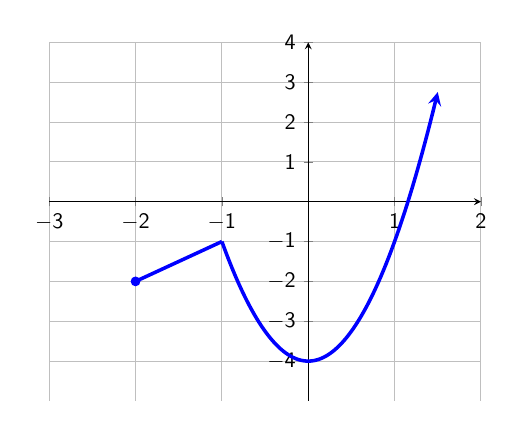
\begin{tikzpicture}[>=stealth, scale=0.8]
    \begin{axis}
    [axis lines = middle, grid,
    xmin = -3, xmax = 2, ymin = -5, ymax = 4,
    % xtick = {-2.5,-2,...,1.5}, 
    ytick = {-4,-3,...,4}
    ]
    \addplot[ultra thick, color=blue,samples=200, domain=-2:-1] {x};
    \addplot[->, ultra thick, color=blue, samples=200, domain=-1:1.5] {3*x^2-4};
    \addplot[color=blue, mark = *] coordinates {(-2,-2)};
    \end{axis}
    \end{tikzpicture}
\end{center}

\begin{multicols}{2}
\begin{enumerate}
\item Domain of $f$
\item Range of $f$
\end{enumerate}	\setcounter{Review}{\value{enumi}}
\end{multicols}
\begin{multicols}{2}
\begin{enumerate}	\setcounter{enumi}{\value{Review}}
\item Relative Minimum
\item Relative Maximum
\end{enumerate}	\setcounter{Review}{\value{enumi}}
\end{multicols}
\begin{multicols}{2}
\begin{enumerate}	\setcounter{enumi}{\value{Review}}
\item $f(1)$
\item $f(0)$
\end{enumerate}	\setcounter{Review}{\value{enumi}}
\end{multicols}
\begin{multicols}{2}
\begin{enumerate}	\setcounter{enumi}{\value{Review}}
\item Increasing Interval(s)
\item Decreasing Interval(s)
\end{enumerate}	\setcounter{Review}{\value{enumi}}
\end{multicols}
\begin{multicols}{2}
\begin{enumerate}	\setcounter{enumi}{\value{Review}}
\item Absolute Maximum
\item Absolute Minimum
\setcounter{Review}{\value{enumi}}
\end{enumerate}
\end{multicols}
\bigskip 

Find each of the following given $f(x) = -2x^{3}+6x^{2}-5x+1$. Round to 3 decimal places and use interval notation when applicable.
\begin{multicols}{4}
\begin{enumerate}
\setcounter{enumi}{\value{Review}}
\item $f(7)$
\item $f(-2)$
\item Rel. Max
\item Rel. Min
\end{enumerate}	\setcounter{Review}{\value{enumi}}
\end{multicols}
\begin{multicols}{4}
\begin{enumerate}	\setcounter{enumi}{\value{Review}}
\item Global Max
\item Global Min
\item Increasing Interval(s)
\item Decreasing Interval(s)
\setcounter{Review}{\value{enumi}}
\end{enumerate}
\end{multicols}
\bigskip 

Use the graph of $f(x)$ to answer each.	\newline\\

\begin{center}
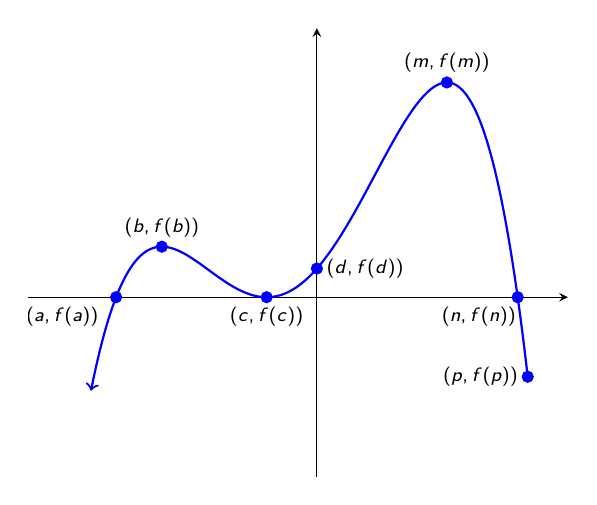
\begin{tikzpicture}[scale=1]
\begin{axis}[
axis lines = middle, xmin = -5.75, xmax = 5, ymin = -10, ymax = 15, ticks=none]
]
\addplot [<-,blue, thick, domain=-4.5:4.2, samples=200] {-0.1*(x+1)*(x+4)*(x+1)*(x-4)};
\addplot[blue, mark=*, only marks] coordinates {(-4,0) (-3.089,2.818) (-1,0) (0,1.6) (2.589,11.975) (4,0) (4.2,-4.434)};
\node at (axis cs: -4,0) [below left, xshift=-0.1cm] {\scriptsize$(a, f(a))$};
\node at (axis cs: -3.089,2.818) [above] {\scriptsize$(b, f(b))$};
\node at (axis cs: -1,0) [below] {\scriptsize$(c, f(c))$};
\node at (axis cs: 0,1.6) [right] {\scriptsize$(d, f(d))$};
\node at (axis cs: 2.589,11.975) [above] {\scriptsize$(m, f(m))$};
\node at (axis cs: 4,0) [below left, xshift=0.1cm] {\scriptsize$(n, f(n))$};
\node at (axis cs: 4.2,-4.434) [left] {\scriptsize$(p, f(p))$};
\end{axis}
\end{tikzpicture}
\end{center}

\begin{multicols}{3}
\begin{enumerate}
\setcounter{enumi}{\value{Review}}
\item Relative maxima of $f(x)$
\item Relative minima of $f(x)$
\item Absolute maxima of $f(x)$
\end{enumerate}	\setcounter{Review}{\value{enumi}}
\end{multicols}
\begin{multicols}{3}
\begin{enumerate}	\setcounter{enumi}{\value{Review}}
\item Absolute minima of $f(x)$
\item Intervals where $f$ is increasing
\item Intervals where $f$ is decreasing
\end{enumerate}	\setcounter{Review}{\value{enumi}}
\end{multicols}
\begin{multicols}{3}
\begin{enumerate}	\setcounter{enumi}{\value{Review}}
\item Zeros of $f$
\end{enumerate} \setcounter{Review}{\value{enumi}}
\end{multicols}

\newpage

Given the labeled points $A$ through $G$ on the graph of $f(x)$ below, find each of the following.  
\begin{center}
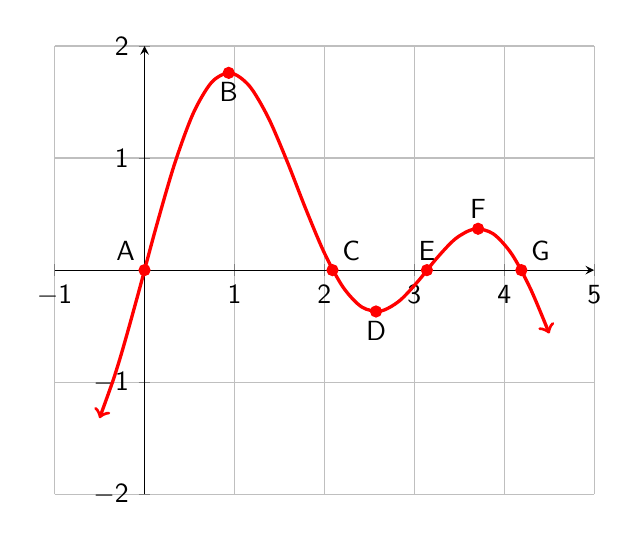
\begin{tikzpicture}
\begin{axis}[
axis lines = middle, xmin = -1, xmax = 5, ymin = -2, ymax = 2, grid
]
\addplot[domain=-0.5:4.5, <->, red, very thick, smooth] {sin(deg(x)) + sin(deg(2*x))};
\coordinate[label = above left: A] (A) at (axis cs:0,0);
\coordinate[label=below:B] (B) at (axis cs:0.936,1.76);
\coordinate[label=above right:C] (C) at (axis cs:2.09,0);
\coordinate[label=below:D] (D) at (axis cs:2.574, -0.369);
\coordinate[label=above:E] (E) at (axis cs:3.14,0);
\coordinate[label=above:F] (F) at (axis cs:3.709,0.369);
\coordinate[label=above right:G] (G) at (axis cs:4.19,0);
\addplot[color=red, mark=*, only marks] coordinates {(0,0) (0.936,1.76) (2.09,0) (2.574, -0.369) (3.14,0) (3.709,0.369) (4.19,0)};
\end{axis}
\end{tikzpicture}
\end{center}

\begin{multicols}{2}
\begin{enumerate}   \setcounter{enumi}{\value{Review}}
    \item Increasing interval(s) 
    \item Decreasing interval(s) 
\end{enumerate}	\setcounter{Review}{\value{enumi}}
\end{multicols}
\begin{multicols}{2}
\begin{enumerate}	\setcounter{enumi}{\value{Review}}
    \item Relative max  
    \item Relative min
\end{enumerate}	\setcounter{Review}{\value{enumi}}
\end{multicols}
\begin{multicols}{2}
\begin{enumerate}	\setcounter{enumi}{\value{Review}}
    \item Global max
    \item Global min
\end{enumerate}	\setcounter{Review}{\value{enumi}}
\end{multicols}
\begin{multicols}{2}
\begin{enumerate}	\setcounter{enumi}{\value{Review}}    
    \item Zeros of $f$  
    \item Number of solutions to $f(x)=1$
\end{enumerate} \setcounter{Review}{\value{enumi}}
\end{multicols}
\bigskip 

Answer each of the following about the function $f(x)$ below.  \newline\\
\begin{center}
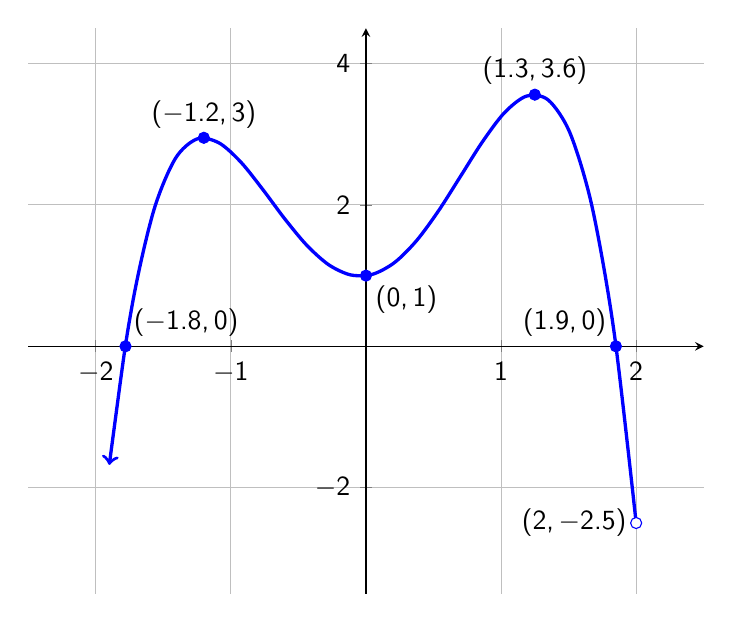
\begin{tikzpicture}
\begin{axis}[width = 4in,
axis lines = middle, xmin = -2.5, xmax = 2.5, ymin = -3.5, ymax = 4.5, grid=major]
\addplot[<-, blue, very thick, domain=-1.9:2, smooth] {-x^4+3*x^2+0.25*x+1};
\addplot[blue, mark=*, only marks] coordinates {(-1.78,0) (-1.2,2.95) (0,1) (1.25,3.56) (1.85,0)};
\addplot[blue, fill=white, mark=*] coordinates {(2,-2.5)};
\node at (axis cs: -1.79,0) [above right] {$(-1.8,0)$};
\node at (axis cs: -1.2,2.95) [above] {$(-1.2,3)$};
\node at (axis cs: 0,1) [below right] {$(0,1)$};
\node at (axis cs: 1.25,3.56) [above] {$(1.3,3.6)$};
\node at (axis cs: 1.85,0) [above left] {$(1.9,0)$};
\node at (axis cs: 2,-2.5) [left] {$(2,-2.5)$};
\end{axis}
\end{tikzpicture}
\end{center}

\begin{multicols}{2}
\begin{enumerate}		\setcounter{enumi}{\value{Review}}
	\item Domain of $f$
    \item Range of $f$
\end{enumerate}	\setcounter{Review}{\value{enumi}}
\end{multicols}
\begin{multicols}{2}
\begin{enumerate}	\setcounter{enumi}{\value{Review}}  
    \item Relative maxima
    \item Relative minima
\end{enumerate}	\setcounter{Review}{\value{enumi}}
\end{multicols}
\begin{multicols}{2}
\begin{enumerate}	\setcounter{enumi}{\value{Review}}  
    \item Absolute maximum
    \item Absolute minimum
\end{enumerate}	\setcounter{Review}{\value{enumi}}
\end{multicols}
\begin{multicols}{2}
\begin{enumerate}	\setcounter{enumi}{\value{Review}}  
    \item Increasing intervals
    \item Decreasing intervals
\end{enumerate}	\setcounter{Review}{\value{enumi}}
\end{multicols}
\begin{multicols}{2}
\begin{enumerate}	\setcounter{enumi}{\value{Review}}  
    \item Zeros of $f(x)$
    \item Number of solutions to $f(x)=2$
\end{enumerate}		\setcounter{Review}{\value{enumi}}
\end{multicols}

\newpage

\section{Answer Key}

\section*{Maxima and Minima}

\begin{enumerate}
	\item Rel max @ $(0,5)$; No rel min
	\item Rel max @ $(2.158, 3.248)$; Rel min @ $(-1.158, -4.048)$
	\item Rel Max $(-1.366,10.848)$ and $(1,6)$; \quad Rel Min $(0.366,5.652)$
    \item Rel Max $(-1.716,11.598)$; \quad Rel Min $(1.132,-3.929)$
    \item Rel Max: $(1.095, 12.096)$; \quad Rel Min $(-0.761, -0.680)$
    \item Rel Max: $(1.366, 0.348)$; \quad
    Rel Min: $(-0.366, -4.848)$ and $(2,0)$
	\item About 2.16 hours
\end{enumerate}

\section*{Increasing, Decreasing, and Constant Intervals}

\begin{enumerate}
	\item Increasing: $(-\infty, 0)$ \quad Decreasing: $(0, \infty)$
	\item Increasing: $(-1.158, 2.158)$ \quad Decreasing: $(-\infty, -1.158) \cup (2.158, \infty)$
    \item Inc: $(-\infty,-2) \cup \left(\frac{2}{3},\infty\right)$ \quad Dec: $\left(-2, \frac{2}{3}\right)$
    \item Inc; $(-1,0) \cup (1, \infty)$ \quad Dec: $(-\infty, -1) \cup (0,1)$
    \item Inc: $(-1,\infty)$ \quad No intervals where it is decreasing
    \item Inc: $(-0.761, 1.095)$; \quad Dec: $(-\infty, -0.761) \cup (1.095, \infty)$
    \item Inc: $(-0.366,1.366) \cup (2, \infty)$; \quad
    Dec: $(-\infty, -0.366) \cup (1.366,2)$;
\end{enumerate}


\section*{Piecewise Functions}
\begin{multicols}{3}
\begin{enumerate}
    \item $\sqrt{15} \approx 3.873$
    \item 7
    \item 6.6
\end{enumerate}	\setcounter{Review}{\value{enumi}}
\end{multicols}
\begin{multicols}{3}
\begin{enumerate}	\setcounter{enumi}{\value{Review}}
    \item 6.4
    \item 7.1
	\item 4
\end{enumerate}	\setcounter{Review}{\value{enumi}}
\end{multicols}
\begin{multicols}{3}
\begin{enumerate}	\setcounter{enumi}{\value{Review}}
    \item $\sqrt{3} \approx 1.732$
    \item 1
    \item 18
\end{enumerate}	\setcounter{Review}{\value{enumi}}
\end{multicols}
\begin{multicols}{3}
\begin{enumerate}	\setcounter{enumi}{\value{Review}}
    \item 17.5
    \item 4
    \item $\frac{5}{8}$
\end{enumerate}	\setcounter{Review}{\value{enumi}}
\end{multicols}
\begin{multicols}{3}
\begin{enumerate}	\setcounter{enumi}{\value{Review}}
    \item 1
    \item $\sqrt{5} \approx 2.236$
    \item $\sqrt{7} \approx 2.646$
\end{enumerate}
\end{multicols}

\newpage

\section*{Miscellaneous}

\begin{multicols}{3}
\begin{enumerate}
    \item $[-2, \infty)$
    \item $[-4, \infty)$
    \item $(0, -4)$
\end{enumerate}	\setcounter{Review}{\value{enumi}}
\end{multicols}
\begin{multicols}{3}
\begin{enumerate}	\setcounter{enumi}{\value{Review}} 
    \item $(-1,-1)$ 
    \item $-1$
    \item $-4)$
\end{enumerate}	\setcounter{Review}{\value{enumi}}
\end{multicols}
\begin{multicols}{3}
\begin{enumerate}	\setcounter{enumi}{\value{Review}} 
    \item $(-2, -1) \cup (0, \infty)$
    \item $(-1,0)$
    \item $(0,-4)$
\end{enumerate}	\setcounter{Review}{\value{enumi}}
\end{multicols}
\begin{multicols}{3}
\begin{enumerate}	\setcounter{enumi}{\value{Review}} 
    \item None
    \item $-426$
    \item 51
\end{enumerate}	\setcounter{Review}{\value{enumi}}
\end{multicols}
\begin{multicols}{3}
\begin{enumerate}	\setcounter{enumi}{\value{Review}} 
    \item (1.408, 0.272)
    \item $(0.592, \, -0.272)$
    \item None
\end{enumerate}	\setcounter{Review}{\value{enumi}}
\end{multicols}
\begin{multicols}{3}
\begin{enumerate}	\setcounter{enumi}{\value{Review}} 
    \item None
    \item $(0.592, \, 1.408)$
    \item $(-\infty, \, 0.592) \cup (1.408, \, \infty)$
\end{enumerate}	\setcounter{Review}{\value{enumi}}
\end{multicols}
\begin{multicols}{3}
\begin{enumerate}	\setcounter{enumi}{\value{Review}} 
	\item $(b, f(b))$ and $(m, f(m))$
	\item $(c, f(c))$
	\item $(m, f(m))$
\end{enumerate}	\setcounter{Review}{\value{enumi}}
\end{multicols}
\begin{multicols}{3}
\begin{enumerate}	\setcounter{enumi}{\value{Review}} 
	\item None
	\item $(-\infty, b) \cup (c, m)$
	\item $(b, c) \cup (m, p)$
\end{enumerate}	\setcounter{Review}{\value{enumi}}
\end{multicols}
\begin{multicols}{3}
\begin{enumerate}	\setcounter{enumi}{\value{Review}} 
	\item $x = a, \, x = c, \, x = n$
    \item $(\infty, B) \cup (D, F)$
    \item $(B, D) \cup (F, \infty)$
\end{enumerate}	\setcounter{Review}{\value{enumi}}
\end{multicols}
\begin{multicols}{3}
\begin{enumerate}	\setcounter{enumi}{\value{Review}} 
    \item $B$ and $F$
    \item $D$
    \item $B$
\end{enumerate}	\setcounter{Review}{\value{enumi}}
\end{multicols}
\begin{multicols}{3}
\begin{enumerate}	\setcounter{enumi}{\value{Review}} 
    \item None
    \item $A, C, E, G$
    \item 2
\end{enumerate}	\setcounter{Review}{\value{enumi}}
\end{multicols}
\begin{multicols}{3}
\begin{enumerate}	\setcounter{enumi}{\value{Review}} 
    \item $(-\infty, 2)$
	\item $(-\infty, -2.5) \cup (-2.5,3.6]$
	\item $(-1.2,3)$ and $(1.3,3.6)$
\end{enumerate}	\setcounter{Review}{\value{enumi}}
\end{multicols}
\begin{multicols}{3}
\begin{enumerate}	\setcounter{enumi}{\value{Review}} 
	\item $(0,1)$
	\item $(1.3,3.6)$
	\item Does not exist
\end{enumerate}	\setcounter{Review}{\value{enumi}}
\end{multicols}
\begin{multicols}{3}
\begin{enumerate}	\setcounter{enumi}{\value{Review}} 
	\item $(-\infty, -1.2) \cup (0,1.3)$
	\item $(-1.2, 0) \cup (1.3,2)$
	\item $(-1.8,0)$ and $(1.9,0)$
\end{enumerate}	\setcounter{Review}{\value{enumi}}
\end{multicols}
\begin{multicols}{3}
\begin{enumerate}	\setcounter{enumi}{\value{Review}} 
	\item 4
\end{enumerate}
\end{multicols}
\chapter{Linear Functions and Slope}

\section{Equations of Lines}

Write the equation of each line \textbf{in point-slope form} that goes through each pair of points.
\begin{enumerate}
\item $(-2, 1), \, (7,8)$
\item $(0,4), \, (9,-15)$
\item $(-1,-2), \, (-3,-13)$
\end{enumerate}

\section{Average Rate of Change}

For the function $f(x) = x^2$, compute the average rate of change for each interval.
\begin{enumerate}
\item $[1, 1.1]$
\item $[1, 1.01]$
\item $[1, 1.001]$
\item $[1,1.0001]$
\setcounter{Review}{\value{enumi}}
\end{enumerate}

\begin{enumerate}
\setcounter{enumi}{\value{Review}}
\item For your answers in the previous four problems, what value do your average rates of change get closer and closer to?
\setcounter{Review}{\value{enumi}}
\end{enumerate}

Find the average rate of change of the function $f(x) = -6x^2 + 7x + 4$ over each specified interval.
\begin{enumerate}
\setcounter{enumi}{\value{Review}}
\item $[-2, -1]$
\item $[5, 6]$
\item $[0, 1]$
\item $[5,5.001]$
\item $[5,5.0001]$
\item $[5,5.00001]$
\item What value are your last 3 answers getting closer to?
\setcounter{Review}{\value{enumi}}
\end{enumerate}

For the function $f(x) = -3x^2 + 5$, determine the average rate of change of each over the given interval.
\begin{enumerate}
\setcounter{enumi}{\value{Review}}
    \item $[7, 7.001]$
    \item $[7, 7.0001]$
    \item $[7, 7.00001]$
\setcounter{Review}{\value{enumi}}
\end{enumerate}

\begin{enumerate}
\setcounter{enumi}{\value{Review}}
\item For your answers in the previous three problems, what value do your average rates of change get closer and closer to?
\setcounter{Review}{\value{enumi}}
\end{enumerate}

\newpage

Given $f(x) = \sqrt{x}$, find the average rate of change of each over the given interval.
\begin{enumerate}
\setcounter{enumi}{\value{Review}}
	\item $[1, 1.0001]$
	\item $[1, 1.00001]$
	\item $[1, 1.000001]$
\setcounter{Review}{\value{enumi}}
\end{enumerate}

\begin{enumerate}
\setcounter{enumi}{\value{Review}}
\item For your answers in the previous three problems, what value do your average rates of change get closer and closer to?
\setcounter{Review}{\value{enumi}}
\end{enumerate}


Given $f(x) = 6\sqrt{x}$, find the average rate of change of each over the given interval.
\begin{enumerate}
\setcounter{enumi}{\value{Review}}
	\item $[25,\, 25.1]$
	\item $[25, \, 25.01]$
	\item $[25, \, 25.001]$
\setcounter{Review}{\value{enumi}}
\end{enumerate}

\begin{enumerate}
\setcounter{enumi}{\value{Review}}
\item For your answers in the previous three problems, what value do your average rates of change get closer and closer to?
\setcounter{Review}{\value{enumi}}
\end{enumerate}

Find the average rate of change of the function $f(x) = -7x^3 + 6\sqrt{3x} + 4$ over each interval. Round your answers to 4 decimal places.
\begin{enumerate}	\setcounter{enumi}{\value{Review}}
	\item $[0,1]$
	\item $[10,11]$
	\item $[8,15]$
\end{enumerate}	\setcounter{Review}{\value{enumi}}

\newpage

\textsc{Linear Functions and Slope Key}

\section*{Equations of Lines}
\begin{enumerate}
\item $y-1 = \frac{7}{9}(x+2)$ \text{ or } $y-8=\frac{7}{9}(x-7)$
    \item $y-4 = -\frac{19}{9}(x-0)$ \text{ or } $y+15=-\frac{19}{9}(x-9)$
    \item $y+2 = \frac{11}{2}(x+1)$ \text{ or } $y+13=\frac{11}{2}(x+3)$
\end{enumerate}

\section*{Average Rate of Change}
\begin{multicols}{3}
\begin{enumerate}
\item 2.1
\item 2.01
\item 2.001
\item 2.0001
\item 2
\item 25
\item $-59$
\item 1
\item $-53.006$
\item $-53.0006$
\item $-53.00006$
\item $-53$
\item $-42.003$
\item $-42.0003$
\item $-42.00003$
\item $-42$
\item $-0.499988$
\item $-0.4999988$
\item $-0.49999988$
\item $-0.5$
\item $0.5994$
\item $0.59999$
\item $0.6$
\item $0.6$
\item 3.3923
\item $-2,315.3960$
\item $-2861.4492$
\end{enumerate}
\end{multicols}
\chapter{Function Transformations}

Write the function for $g(x)$ if it is the result of $f(x)$ after the following ordered sequence of transformations.
\begin{enumerate}
\item \begin{enumerate}[(1)]
	\item Vertical stretch by 3
	\item Shift left 1 unit
	\item Reflect across $y$-axis
\end{enumerate}
\item \begin{enumerate}[(1)]
	\item Horizontal compression by 2
	\item Shift up 1 unit
\end{enumerate}
\item \begin{enumerate}[(1)]
	\item Reflect across $x$-axis
	\item Vertical compression by 4
	\item Move right 7 units
\end{enumerate}
\setcounter{Review}{\value{enumi}}
\end{enumerate}

Write the function $g(x)$ that is a result of the following ordered sequence of transformations to $f(x)=|x|$.
\begin{enumerate}
\setcounter{enumi}{\value{Review}}
\item
\begin{enumerate}[(1)]
\item Reflect across $x$-axis
\item Shift right 3 units
\item Horizontal stretch by factor of 5
\end{enumerate}

\item
\begin{enumerate}[(1)]
\item Shift down 2 units
\item Reflect across $y$-axis
\item Shift up 1 unit
\end{enumerate}

\item
\begin{enumerate}[(1)]
\item Horizontal compression by factor of 7
\item Vertical compression by factor of 4
\item Shift left 9 units
\end{enumerate}
\setcounter{Review}{\value{enumi}}
\end{enumerate}

Given $f(x) = \sqrt{x}$, determine the resulting function $g(x)$ after the following ordered sequence of transformations.
\begin{enumerate}
\setcounter{enumi}{\value{Review}}
\item
\begin{enumerate}[(1)]
\item Shift up 2 units
\item Horizontal stretch by 5
\item Shift left 3 units
\end{enumerate}

\item
\begin{enumerate}[(1)]
\item Vertical compression by factor of 3
\item Reflect across $y$-axis
\item Horizontal compression by 5
\end{enumerate}

\item
\begin{enumerate}[(1)]
\item Shift right 8 units
\item Reflect across $x$-axis
\item Horizontal compression by factor of 4
\end{enumerate}
\setcounter{Review}{\value{enumi}}
\end{enumerate}

\newpage

Write the final equation of $g(x)$ if it is found by taking $f(x) = \sqrt{x}$ after the following ordered sequence of transformations.   

\begin{enumerate}	\setcounter{enumi}{\value{Review}}
\item \begin{enumerate}[(1)]
\setlength\itemsep{0pt}
    \item Shift right 2 units
    \item Horizontal stretch by factor 3
    \item Shift down 2 units
    \item Reflect across $x$-axis
\end{enumerate}

\item
\begin{enumerate}[(1)]
\setlength\itemsep{0pt}
    \item Horizontal stretch by factor 3
    \item Shift left 1 unit
    \item Shift up 2 units
    \item Reflect across $y$-axis
\end{enumerate}

\item
\begin{enumerate}[(1)]
\setlength\itemsep{0pt}
    \item Vertical stretch by factor 5
    \item Horizontal stretch by factor 2
    \item Shift up 3 units
    \item Reflect across $x$-axis
\end{enumerate}
\setcounter{Review}{\value{enumi}}
\end{enumerate}

Find the equation for $g(x)$ if $g(x)$ is found by performing the following \emph{ordered} sequence of transformations to $f(x)=\frac{1}{x}$.

\begin{enumerate}	\setcounter{enumi}{\value{Review}}
\item \begin{enumerate}[(1)]
\setlength\itemsep{0pt}
	\item Shift left 3 spaces
	\item Reflect across $y$-axis
	\item Shift down 5 spaces
	\item Vertical stretch by factor of 7
\end{enumerate}
\setcounter{Review}{\value{enumi}}
\end{enumerate}

\begin{enumerate}	\setcounter{enumi}{\value{Review}}
\item \begin{enumerate}[(1)]
\setlength\itemsep{0pt}
	\item Shift up 3 spaces
	\item Reflect across $x$-axis
	\item Shift right 5 spaces
	\item Horizontal compression by factor of 7
\end{enumerate}
\setcounter{Review}{\value{enumi}}
\end{enumerate}

Given the graph of $f(x)$ below, find the new coordinates of each point after the following transformations.
\begin{center}
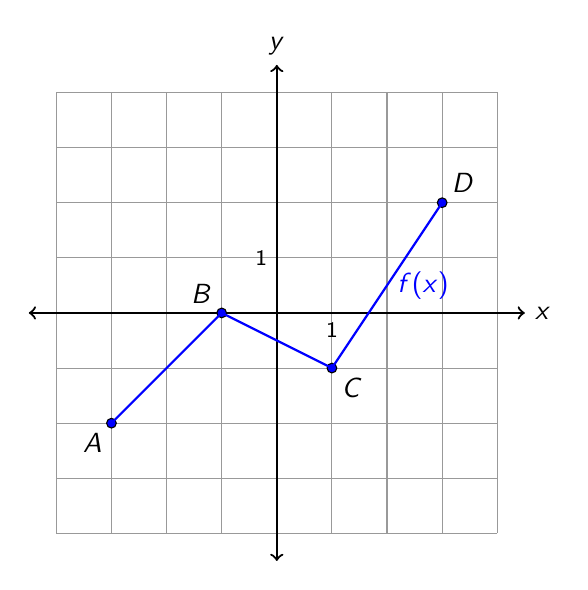
\begin{tikzpicture}[scale=0.7]
\draw[gray!80] (-4,-4) grid (4,4);
\draw[<->, thick] (-4.5,0) -- (4.5,0) node [right] {$x$};
\draw[<->, thick] (0,-4.5) -- (0,4.5) node [above] {$y$};
\coordinate (A) at (-3,-2);
\coordinate (B) at (-1,0);
\coordinate (C) at (1,-1);
\coordinate (D) at (3,2);
\draw[fill=blue] (A) circle [radius=2.5pt] node [below left] {$A$};
\draw[fill=blue] (B) circle [radius=2.5pt] node [above left] {$B$};
\draw[fill=blue] (C) circle [radius=2.5pt] node [below right] {$C$};
\draw[fill=blue] (D) circle [radius=2.5pt] node [above right] {$D$};
\draw[thick,blue] (A) -- (B) -- (C) -- node [midway, right] {$f(x)$} (D);
\node at (1,0) [below] {\footnotesize 1};
\node at (0,1) [left] {\footnotesize 1};
\end{tikzpicture}
\end{center}

\begin{enumerate} \setcounter{enumi}{\value{Review}}
    \item $-2f(x+1)$ 
    \item $f\left(-\frac{1}{2}x\right)-3$
    \item $\frac{1}{2}f(-x-2)+2$
    \item $f(2x+2)-1$
\setcounter{Review}{\value{enumi}}
\end{enumerate}

\newpage

\textsc{Function Transformations Key} 

\begin{enumerate}
	\item $g(x) = 3f(-x+1)$
	\item $g(x) = f(2x)+1$
	\item $g(x) = -\frac{1}{4}f(x-7)$
    \item $g(x) = -\left|\frac{1}{5}x-3\right|$
    \item $g(x) = |-x|-1$
    \item $g(x) = \frac{1}{4}|7(x+9)| = \frac{1}{4}|7x+63|$
    \item $g(x) = \sqrt{\frac{1}{5}(x+3)} + 2 = \sqrt{\frac{1}{5}x + \frac{3}{5}}+2$
    \item $g(x) = \frac{1}{3}\sqrt{-5x}$
    \item $g(x) = -\sqrt{4x-8}$
    \item $g(x) = -\left(\sqrt{\frac{1}{3}x-2}-2\right) = -\sqrt{\frac{1}{3}x-2}+2$
    \item $g(x) = \sqrt{\frac{1}{3}(-x+1)}+2 = \sqrt{-\frac{1}{3}x+\frac{1}{3}}+2$
    \item $g(x) = -\left(5\sqrt{\frac{1}{2}x}+3\right) = -5\sqrt{\frac{1}{2}x} - 3$
    \item $g(x) = \frac{7}{-x+3} - 35$
    \item $g(x) = -\frac{1}{7x-5} - 3$ 
    \item $A'(-4,4), \, B'(-2,0), \, C'(0,2), \, D'(2,-4)$
    \item $A'(6,-5), \, B'(2,-3), \, C'(-2, -4), \, D'(-6,-1)$
    \item $A'(1,1), \, B'(-1,2), \, C'(-3,1.5), \, D'(-5,3)$
    \item $A'(-2.5,-3), \, B'(-1.5,-1), \, C'(-0.5,-2), \, D'(0.5,1)$
\end{enumerate}

\chapter{Function Operations}

\section{Adding, Subtracting, Multiplying, and Dividing Functions}

Given $f(x) = x + 5$, $g(x) = x^2 - 1$, and $h(x) = \sqrt{x-10}$, simplify or evaluate each.
\begin{enumerate}
    \item $(g-f)(x)$
    \item $(fh)(14)$
    \item $(f+g)(x)$
\end{enumerate}

\section{Operations with Functions: Domain}

Given $f(x)=\sqrt{2x+7}$ and $g(x) = 3x+3$, find the domain of each.
\begin{enumerate}
\item $(f + g)(x)$
\item $\left(\frac{f}{g}\right)(x)$
\item $\left(\frac{g}{f}\right)(x)$
\end{enumerate}


\section{Difference Quotient}

Write the difference quotient for each.
\begin{enumerate}
	\item $f(x) = 2x - 7$
	\item $g(x) = x^2 + 4x$
	\item $h(x) = -1$
	\item $f(x) = \frac{3}{x+2}$
	\item $g(x) = \sqrt{3x}$
	\item $f(x) = x^2 - 2x + 5$
	\item $g(x) = \frac{5}{x}$
\end{enumerate}


\newpage


\textsc{Function Operations Key}

\section*{Adding, Subtracting, Multiplying, and Dividing Functions}

\begin{enumerate}
    \item $x^2-x-6$
    \item 38
    \item $x^2+x+4$
\end{enumerate}

\section*{Operations with Functions: Domain}
\begin{enumerate}
	\item $\left[-\frac{7}{2}, \infty\right)$
    \item $\left[-\frac{7}{2}, -1\right) \cup (-1, \infty)$
    \item $\left(-\frac{7}{2}, \infty\right)$
\end{enumerate}

\section*{Difference Quotient}

\begin{enumerate}
	\item 2
	\item $2x + h + 4$
	\item 0
    \item $\frac{-3}{(x+2)(x+h+2)}$
    \item $\frac{3}{\sqrt{3x+3h}+\sqrt{3x}}$
    \item $2x+h-2$
    \item $\frac{-5}{x(x+h)}$
\end{enumerate}
\chapter{Polynomials and Their Graphs}

Find the degree, leading term, leading coefficient, and constant term of the following polynomials.
\begin{multicols}{3}
\begin{enumerate}
\item $f(x) = -x^5 + \sqrt{7}x^3 - 2x^2$
\item $g(x) = 4x^2 - 16x^6 + 3x$
\item $h(x) = 1 + x^{11} - 4x^8$
\end{enumerate}	\setcounter{Review}{\value{enumi}}
\end{multicols}
\begin{multicols}{3}
\begin{enumerate}	\setcounter{enumi}{\value{Review}} 
\item $f(x) = -x^4+3x^2-2x+6$
\item $g(x) = 0.25x^5-0.1x^4+2x^2-6x$
\item $f(x) = -6x^3 + 2x^2 + 7x^4 - 1$
\end{enumerate}	\setcounter{Review}{\value{enumi}}
\end{multicols}
\begin{multicols}{3}
\begin{enumerate}	\setcounter{enumi}{\value{Review}} 
\item $g(x) = \frac{1}{3}x^3 - \frac{\pi}{8}x^2 + x\sqrt{2} - 3^4$
\item $h(x) = 7(x+1)^2(x-2)^3$
\item $j(x) = -\frac{1}{2}\left(3x+2\right)^2(x-1)^5$
\end{enumerate}		\setcounter{Review}{\value{enumi}}
\end{multicols}
\bigskip

Determine the end behavior of each.
\begin{multicols}{3}
\begin{enumerate}	\setcounter{enumi}{\value{Review}}
\item $f(x) = -x^5 + \sqrt{7}x^3 - 2x^2$
\item $g(x) = 4x^2 - 16x^6 + 3x$
\item $h(x) = 1 + x^{11} - 4x^8$
\end{enumerate}	\setcounter{Review}{\value{enumi}}
\end{multicols}
\begin{multicols}{3}
\begin{enumerate}	\setcounter{enumi}{\value{Review}} 
\item $f(x) = -x^4+3x^2-2x+6$
\item $g(x) = 0.25x^5-0.1x^4+2x^2-6x$
\item $f(x) = -6x^3 + 2x^2 + 7x^4 - 1$
\end{enumerate}	\setcounter{Review}{\value{enumi}}
\end{multicols}
\begin{multicols}{3}
\begin{enumerate}	\setcounter{enumi}{\value{Review}} 
\item $g(x) = \frac{1}{3}x^3 - \frac{\pi}{8}x^2 + x\sqrt{2} - 3^4$
\item $h(x) = 5(x+1)^2(x-2)^3$
\item $j(x) = -\frac{1}{2}\left(3x+2\right)^2(x-1)^5$
\end{enumerate}	\setcounter{Review}{\value{enumi}}
\end{multicols}
\bigskip

Find the zeros of each. Round to 2 decimal places when necessary.
\begin{multicols}{3}
\begin{enumerate}	\setcounter{enumi}{\value{Review}}
\item $f(x) = -x^5 + \sqrt{7}x^3 - 2x^2$
\item $g(x) = 4x^2 - 16x^6 + 3x$
\item $h(x) = 1 + x^{11} - 4x^8$
\end{enumerate}	\setcounter{Review}{\value{enumi}}
\end{multicols}
\begin{multicols}{3}
\begin{enumerate}	\setcounter{enumi}{\value{Review}} 
\item $f(x) = -x^4+3x^2-2x+6$
\item $g(x) = 0.25x^5-0.1x^4+2x^2-6x$
\item $f(x) = -6x^3 + 2x^2 + 7x^4 - 1$
\end{enumerate}	\setcounter{Review}{\value{enumi}}
\end{multicols}
\begin{multicols}{3}
\begin{enumerate}	\setcounter{enumi}{\value{Review}} 
\item $g(x) = \frac{1}{3}x^3 - \frac{\pi}{8}x^2 + x\sqrt{2} - 3^4$
\item $h(x) = 5(x+1)^2(x-2)^3$
\item $j(x) = -\frac{1}{2}\left(3x+2\right)^2(x-1)^5$
\end{enumerate}	\setcounter{Review}{\value{enumi}}
\end{multicols}

\newpage

\section{Answer Key}

\begin{enumerate}
	\item Degree = 5, Leading Term = $-x^5$, Leading Coefficient = $-1$, Constant = none (or 0)
	\item Degree = 6, Leading Term = $-16x^6$, Leading Coefficient = $-16$, Constant = none (or 0)
	\item Degree = 11, Leading Term = $x^{11}$, Leading Coefficient = 1, Constant = 1
	\item Degree = 4, Leading Term = $-x^4$, Leading Coefficient = $-1$, Constant = 6
	\item Degree = 5, Leading Term = $0.25x^5$, Leading Coefficient = $0.25$, Constant = none (or 0)
	\item Degree = 3, Leading Term = $-6x^3$, Leading Coefficient = $-6$, Constant = $-1$
	\item Degree = 3, Leading Term = $\frac{1}{3}x^3$, Leading Coefficient = $\frac{1}{3}$, Constant = $3^4$
	\item Degree = 5, Leading Term = $7x^5$, Leading Coefficient = 7, Constant = $-56$
	\item Degree = 7, Leading Term = $-\frac{9}{2}x^7$, Leading Coefficient = $-\frac{9}{2}$, Constant = 2
	\item $\displaystyle \lim_{x \to -\infty} f(x) = \infty \quad \lim_{x \to \infty}f(x) = -\infty$
	\item $\displaystyle \lim_{x \to -\infty} g(x) = -\infty, \quad \lim_{x \to \infty}g(x) = \infty$
	\item $\displaystyle \lim_{x \to -\infty} h(x) = -\infty \quad \lim_{x \to \infty}h(x) =\infty$
	\item $\displaystyle \lim_{x \to -\infty}f(x) = -\infty$ \quad $\lim_{x \to \infty}f(x) = -\infty$
    \item $\displaystyle \lim_{x \to -\infty}g(x) = -\infty$ \quad $\lim_{x \to \infty}g(x) = \infty$
    \item $\displaystyle \lim_{x \to -\infty} f(x) = \infty \quad \lim_{x \to \infty} f(x) = - \infty$
    \item $\displaystyle \lim_{x \to -\infty} g(x) = -\infty \quad \lim_{x \to \infty} g(x) = \infty$
    \item $\displaystyle \lim_{x \to -\infty} h(x) = -\infty \quad \lim_{x \to \infty} h(x) = \infty$
     \item $\displaystyle \lim_{x \to -\infty} j(x) = \infty \quad \lim_{x \to \infty} j(x) = -\infty$
     \item $(-1.92,0), \, (0,0)$
     \item $(0,0), \, (0.83,0)$
     \item $(-0.83,0), \, (0.86,0), \, (1.58,0)$
     \item $(-2.25,0), \, (1.90,0)$
     \item $(-2.48,0), \, (0,0), \, (1.85,0)$
     \item $(-0.42,0), \, (0.79,0)$
     \item $(6.42,0)$
     \item $(-1,0), \, (2,0)$
     \item $\left(-\frac{2}{3},0\right), \, (1,0)$
\end{enumerate}
\chapter{Dividing Polynomials}

\section{Dividing Polynomials}

Divide each.
\begin{enumerate}
    \item $(28x^3-26x^2+41x-15) \div (7x-3)$
    \item $(44y^2+12y^3+61y-37) \div (3y+5)$
    \item $\left(4x^3 - 3x^2 + x + 1\right) \div (x + 2)$
    \item $\left(5x^4 - x^2 + x - 2\right) \div (x^2 + 2)$
\end{enumerate}

\section{Remainder and Factor Theorems}

Determine the remainder of each.
\begin{enumerate}
	\item $\left(2x^{53} - 9x^{44} + 13x^8\right) \div (x - 1)$
	\item $\left(x^{71} + 15x^{58} - 3x^{14} + 2\right) \div (x + 1)$
\end{enumerate}

\newpage

\textsc{Dividing Polynomials Key}

\section*{Dividing Polynomials}

\begin{enumerate}
    \item $4x^2-2x+5$
    \item $4y^2+8y+7-\frac{72}{3y+5}$
    \item $4x^2 - 11x + 23 - \frac{45}{x+2}$
    \item $5x^2 - 11 + \frac{x+20}{x^2+2}$
\end{enumerate}

\section*{Remainder and Factor Theorems}

\begin{enumerate}
	\item 6
	\item 13
\end{enumerate}
\chapter{Rational Functions and Their Graphs}

Find the domain, coordinates of any holes, and equations of all asymptotes.
\begin{enumerate}
\setlength\itemsep{10pt}
	\item $f(x) = \frac{2x^2+5x-3}{2x^2-15x+7}$
	\item $g(x) = \frac{3x^3+7x^2-20x}{x^2-x-12}$
	\item $f(x) = \frac{3x}{x+4}$
	\item $g(x) = \frac{x^2+3x+2}{x-1}$
	\item $h(x) = \frac{x^2+3x-4}{x^3-2x^2+x}$
	\item $f(x) = \frac{2x^3-13x^2+6x+45}{x^2-4x-5}$
	\item $g(x) = \frac{5x^2-19x-4}{x^3+2x^2-24x}$
	\item $h(x) = \frac{2x^2-x-3}{8x^2+51x+18}$
	\item $f(x) = \frac{6x^3 - 21x^2 - 51x + 30}{3x^2+7x+2}$
	\item $g(x) = \frac{10x^2-29x-21}{10x^3-33x^2-7x}$
\end{enumerate}	\setcounter{Review}{\value{enumi}}

State the end behavior of each.
\begin{enumerate}	\setcounter{enumi}{\value{Review}}
	\item $k(x) = \frac{5x^3-7x^2+8}{-3x^3+6x-4}$
	\item $m(x) = \frac{2x-1}{3x^2+7x+1}$
\end{enumerate}

\newpage

\textsc{Rational Functions and Their Graphs Key}

\begin{enumerate}
    \item Domain: $x \neq -\frac{1}{2}, \, 7$; V.A.: $x=7$; Hole @ $\left(-\frac{1}{2},-\frac{7}{13}\right)$; H.A.: $y=1$
    \item Domain: $x \neq -3, \, 4$; V.A.: $x=-3 \, x = 4$; Obl. Asymp: $y = 3x+10$
    \item Domain: $x \neq -4$; V.A.: $x = -4$; H.A.: $y = 3$
    \item Domain: $x \neq 1$; V.A.: $x = 1$; Obl. Asymp: $y = x + 4$
    \item Domain: $x \neq 0, 1$; V.A.: $x = 0$ and $x = 1$; H.A.: $y = 0$ 
    \item Domain: $x \neq -1, 5$; V.A. $x=-1$; Hole @ $\left(5, \frac{13}{3}\right)$; Obl. Asym $y = 2x-5$
    \item Domain: $x \neq -6, 0, 4$; V.A. $x = -6, \, x = 0$; Hole @ $\left(4, \frac{21}{40}\right)$; H.A. $y = 0$
    \item Domain: $x \neq -6, -\frac{3}{8}$; V.A. $x = -6, \, x = -\frac{3}{8}$; H.A. $y = \frac{1}{4}$
    \item Domain: $x \neq -2, \, -\frac{1}{3}$; Hole @ $(-2,-21)$; V.A.: $x = -\frac{1}{3}$; S.A. $y = 2x-\frac{35}{3}$
    \item Domain: $x \neq -\frac{1}{5}, \, 0, \, \frac{7}{2}$; Hole @ $\left(\frac{7}{2}, \frac{82}{259}\right)$; V.A. $x = -\frac{1}{5}$ and $x=0$; H.A. $y=0$
    
%%%%% End Behavior %%%%%%%%%
    \item $\lim_{x \to -\infty} k(x) = \infty = \lim_{x \to \infty} k(x) = -\frac{5}{3}$
    \item $\lim_{x \to -\infty} m(x) = \infty = \lim_{x \to \infty} m(x) = 0$
\end{enumerate}
\chapter{Polynomial and Rational Inequalities}

\section{Polynomial Inequalities}

Solve each. Write your answers using interval notation.
\begin{enumerate}
\item $6x^3-4x^2-10x \geq 0$
\end{enumerate}

\section{Rational Inequalities}

Solve each. Write your answers using interval notation.
\begin{enumerate}
\setlength\itemsep{10pt}
\item $\frac{3x-4}{x+1}<0$
\item $\frac{x^2+3x+2}{x-7} \leq 0$
\end{enumerate}

\newpage

\textsc{Polynomial and Rational Inequalities Key}

\section*{Polynomial Inequalities}
\begin{enumerate}
    \item $[-1,0] \cup \left[\frac{5}{3}, \infty\right)$
\end{enumerate}
\section*{Rational Inequalities}
\begin{enumerate}
    \item $\left(-1, \frac{4}{3}\right)$
    \item $(-\infty,-2] \cup [-1, 7)$
\end{enumerate}
\chapter{Function Compositions}

Given $f(x) = x - 5$, $g(x) = 4 + \sqrt{2x+1}$, and $h(x) = \dfrac{3}{x+7}$, simplify each \underline{and state the domain}.
\begin{enumerate}
	\item $(f \circ g)(x)$
	\item $(g \circ f)(x)$
	\item $h(h(x))$
\setcounter{Review}{\value{enumi}}
\end{enumerate}

Find each of the following given the table below.
\begin{center}
\begin{tabular}{c|c|c|c|c|c|c|c|c|c}
    $\bm{x}$ & $\bm{-4}$ & $\bm{-3}$ & $\bm{-2}$ & $\bm{-1}$ & \textbf{0} & \textbf{1} & \textbf{2} & \textbf{3} & \textbf{4} \\ \hline
    $\bm{f(x)}$ & $-3$ & 0 & $-1$ & 3 & 1 & 2 & 4 & $-4$ & $-2$ \\ \hline
    $\bm{g(x)}$ & 3 & $-1$ & 0 & 1 & 4 & $-2$ & $-4$ & 2 & $-3$ \\
\end{tabular}
\end{center}

\begin{multicols}{5}
\begin{enumerate}	\setcounter{enumi}{\value{Review}}
\item $(f \circ g)(-1)$
\item $(g \circ g)(0)$
\item $(f \circ f)(2)$
\item $(g \circ g)(-3)$
\item $f(g(0))$
\setcounter{Review}{\value{enumi}}
\end{enumerate}
\end{multicols}

Given $f(x) = \sqrt{3x+2}$, $g(x) = x^2 - 1$, and $h(x) = 9x-2$, find each of the following.
\begin{enumerate}
\setcounter{enumi}{\value{Review}}
\item $(g \circ f)(x)$
\item $f(g(x))$
\item $(h \circ h)(x)$
\setcounter{Review}{\value{enumi}}
\end{enumerate}

\newpage

\textsc{Function Compositions Key}

\begin{enumerate}
	\item $-1 + \sqrt{2x+1}$ Domain: $\left[-\frac{1}{2}, \infty\right)$
	\item $4 + \sqrt{2x-9}$ Domain: $\left[\frac{9}{2}, \infty\right)$
	\item $\frac{3x+21}{7x+52}$ Domain: $\left(-\infty, -\frac{52}{7}\right) \cup \left(-\frac{52}{7}, -7\right) \cup (-7, \infty)$
	\item 2
     \item $-3$
     \item $-2$
     \item 1
     \item $-2$
     \item $3x + 1$
    \item $\sqrt{3x^2-1}$
    \item $81x-20$
\end{enumerate}
\chapter{Inverse Functions}

Find the inverse of each. Then state the domain and range of the function and the inverse.

\begin{enumerate}
	\item $f(x) = \sqrt{-2x + 3} + 1$
	\item $g(x) = (x+4)^2 - 1, \, x \leq -4$
	\item $h(x) = \frac{9x}{4x-1}$
	\item $f(x) = \sqrt{x} - 3$
	\item $g(x) = \frac{1}{1-x}$
	\item $h(x) = x^2 + 6x + 4, \, x \leq -3$
	\item $f(x) = \sqrt{5x-4}$
	\item $g(x) = x^2 - 2x + 3, \, x \leq 1$
	\item $h(x) = \frac{3}{x-1}$
	
	\item $f(x) = 5-\sqrt{2x}$
    \item $g(x) = \frac{5}{x+1}$
    \item $h(x) = \frac{3x}{x-2}$
\end{enumerate}

\newpage

\section{Answer Key}

\begin{enumerate}
	\item $f^{-1}(x) = -\frac{1}{2}\left((x-1)^2-3\right)$ \newline\\
     \begin{tabular}{c|c|c}
         &   Domain  &   Range   \\  \hline
         $f(x)$ & $(-\infty, 1.5]$ & $[1, \infty)$ \\ \hline
         $f^{-1}(x)$ & $[1, \infty)$ & $(-\infty, 1.5]$ \\ 
     \end{tabular}
     
     \item $g^{-1}(x) = -\sqrt{x+1}-4$   \newline\\
     \begin{tabular}{c|c|c}
         &   Domain  &   Range   \\  \hline
         $g(x)$ & $(-\infty, -4]$ & $[-1, \infty)$ \\ \hline
         $g^{-1}(x)$ & $[-1, \infty)$ & $(-\infty, -4]$ \\ 
     \end{tabular}
     
     \item $h^{-1}(x) = \frac{-x}{9-4x}$ \newline\\
     \begin{tabular}{c|c|c}
         &   Domain  &   Range   \\  \hline
         $h(x)$ & $(-\infty, 1/4) \cup (1/4, \infty) $ & $(\infty, 9/4) \cup (9/4, \infty)$ \\ \hline
         $h^{-1}(x)$ & $(\infty, 9/4) \cup (9/4, \infty)$ & $(-\infty, 1/4) \cup (1/4, \infty) $ \\ 
     \end{tabular}
         
     \item $f^{-1}(x) = (x+3)^2$ \newline\\
	\begin{tabular}{c|c|c}
            &   Dom             &   Ran \\  \hline
    $f(x)$  &   $[0,\infty)$    &   $[-3,\infty)$   \\  \hline
    $f^{-1}(x)$ &   $[-3,\infty)$   &   $[0,\infty)$    \\
\end{tabular}
     
     \item $g^{-1}(x) = 1 - \frac{1}{x}$  \newline\\
\begin{tabular}{c|c|c}
            &   Dom             &   Ran \\  \hline
    $g(x)$  &   $(-\infty,1)\cup(1,\infty)$    &   $(-\infty,0)\cup(0,\infty)$   \\  \hline
    $g^{-1}(x)$ &   $(-\infty,0)\cup(0,\infty)$   &   $(-\infty,1)\cup(1,\infty)$    \\
\end{tabular}

\item $h^{-1}(x) = -\sqrt{x+5}-3$ \newline\\ 
\begin{tabular}{c|c|c}
            &   Dom             &   Ran \\  \hline
    $h(x)$  &   $(-\infty,-3]$    &   $[-5,\infty)$   \\  \hline
    $h^{-1}(x)$ &   $[-5,\infty)$   &   $(-\infty,-3]$    \\
\end{tabular}

\item $f^{-1}(x) = \frac{1}{5}x^2 + \frac{4}{5}$    \newline\\
    \setlength{\extrarowheight}{5pt}
    \begin{tabular}{c|c|c}
            &   Dom &   Ran \\  \hline
        $f(x)$  &   $\left[\frac{4}{5}, \infty\right)$  &   $[0, \infty)$    \\[5pt]  \hline
        $f^{-1}(x)$ &   $[0, \infty)$   &   $\left[\frac{4}{5}, \infty\right)$  \\
    \end{tabular}
    
\item $g^{-1}(x) = -\sqrt{x-2}+1$   \newline\\
    \setlength{\extrarowheight}{5pt}
    \begin{tabular}{c|c|c}
            &   Dom &   Ran \\  \hline
        $g(x)$  &   $(-\infty, 1]$  &   $[2, \infty)$    \\[5pt]  \hline
        $g^{-1}(x)$ &   $[2, \infty)$   &   $(-\infty, 1]$  \\
    \end{tabular}
    
\item $h^{-1}(x) = \frac{3}{x} + 1$ \newline\\
    \setlength{\extrarowheight}{5pt}
    \begin{tabular}{c|c|c}
            &   Dom &   Ran \\  \hline
        $h(x)$  &   $(-\infty, 1) \cup (1, \infty)$  &   $(-\infty, 0) \cup (0, \infty)$    \\[5pt]  \hline
        $h^{-1}(x)$ &   $(-\infty, 0) \cup (0, \infty)$   &   $(-\infty, 1) \cup (1, \infty)$  \\
        \end{tabular}
        
\newpage 
        
\item $f^{-1}(x) = \frac{1}{2}(x-5)^2; \, x \leq 5$ \newline\\
    
    \begin{tabular}{c|c|c}
                    &   Domain      & Range             \\ \hline
        $f(x)$      & $[0,\infty)$  &   $(-\infty, 5]$  \\  \hline   
        $f^{-1}(x)$ & $(-\infty,5]$ &   $[0,\infty)$  
    \end{tabular}
    
    \item $g^{-1}(x) = \frac{5}{x}-1$   \newline\\
    
    \begin{tabular}{c|c|c}
                    &   Domain      & Range             \\ \hline
        $g(x)$      & $(-\infty,-1)\cup(-1,\infty)$  &   $(-\infty,0)\cup(0,\infty)$  \\  \hline   
        $g^{-1}(x)$ & $(-\infty,0)\cup(0,\infty)$ &   $(-\infty,-1)\cup(-1,\infty)$  
    \end{tabular}
    
    \item $h^{-1}(x) = \frac{2x}{x-3}$    \newline\\
    
    \begin{tabular}{c|c|c}
                    &   Domain      & Range             \\ \hline
        $h(x)$      & $(-\infty,2)\cup(2,\infty)$  &   $(-\infty,3)\cup(3,\infty)$  \\  \hline   
        $h^{-1}(x)$ & $(-\infty,3)\cup(3,\infty)$ &   $(-\infty,2)\cup(2,\infty)$  
    \end{tabular}

    



\end{enumerate}
\chapter{Exponential Functions}

\section{End Behavior}

Determine the end behavior of each. Write your answers using limit notation.
\begin{enumerate}
	\item $f(x) = 3 + e^{2x}$
	\item $h(x) = 5^{-x}$
	\item $h(x) = -\frac{2}{3}e^{x+7} + 1$
\end{enumerate}

\newpage

\textsc{Exponential Functions}

\begin{enumerate}
	\item $\lim_{x \to -\infty} f(x) = 3$ \quad $\lim_{x \to \infty} f(x) = \infty$
	\item $\lim_{x \to -\infty} f(x) = \infty$ \quad $\lim_{x \to \infty} f(x) =0$ 
	\item $\lim_{x \to -\infty} h(x) = 0 \quad \lim_{x \to \infty} h(x) = - \infty$
\end{enumerate}

\chapter{Logarithmic Functions}

Find the domain of each. Write your answers in interval notation.
\begin{enumerate}
	\item $b(x) = \log_7\left(x^2 - 8x + 6\right)$
	\item $a(x) = \ln\left(\frac{x^2+3x+2}{5x+15}\right)$
	\item $f(x) = -7\ln\left(x^2 + 9x + 8\right)$
	\item $g(x) = \log\left(5x^2 + 13x - 6\right)$
	\item $h(x) = 3\log_2\left(x^3+2x^2-x-2\right)$
\end{enumerate}
\setcounter{Review}{\value{enumi}}

State the end behavior of each.
\begin{enumerate}	\setcounter{enumi}{\value{Review}}
	\item $j(x) = 5\log_3\left(2x-5\right) - 2$
\end{enumerate}

\newpage

\textsc{Logarithmic Functions Key}

\begin{enumerate}
	\item $(-\infty, 0.838) \cup (7.162, \infty)$
    \item $(-3, -2) \cup (-1, \infty)$
    \item $(-\infty, -8) \cup (-1, \infty)$
    \item $(-\infty, -2) \cup \left(-\frac{3}{5}, \infty\right)$
    \item $(-2, -1) \cup (1, \infty)$
    \item $\lim_{x \to (5/2)^+} j(x) = -\infty \quad \lim_{x \to \infty} j(x) = \infty$ 
\end{enumerate}

\chapter{Properties of Logarithms}

Expand or condense each completely. Simplify numerical answers.
\begin{enumerate}
	\item $\log_b\left(\frac{x^2}{y^8}\right)$
	\item $\ln\left(ez\right)^3$
	\item $\log_5(x) + \log_5(9) - 2\log_5(w)$
\setcounter{Review}{\value{enumi}}
\end{enumerate}

Write an equivalent expression for each of the following using natural logarithms.
\begin{enumerate}
\setcounter{enumi}{\value{Review}}
	\item $\log_7(10)$
	\item $\log_9(x)$
	\item $\log_b(c)$
\setcounter{Review}{\value{enumi}}
\end{enumerate}

Suppose that $\log_a(b) = 5, \, \log_a(c) = 12, \text{ and } \log_a(d) = 9$. Evaluate each of the following.
\begin{enumerate}	\setcounter{enumi}{\value{Review}}
	\item $\log_a(bc)$
    \item $\log_a(c^3)$
    \item $\log_a\left(\frac{d}{c}\right)$
    \item $\log_a\left(\frac{bd}{c}\right)$
\end{enumerate}
\setcounter{Review}{\value{enumi}}

\newpage

\textsc{Properties of Logarithms Key}

\begin{enumerate}
	\item $2\log_b(x) - 8\log_b(y)$
    \item $3 + 3\ln(z)$
    \item $\log_5\left(\frac{9x}{w^2}\right)$
    \item $\frac{\ln(10)}{\ln(7)}$
    \item $\frac{\ln(x)}{\ln(9)}$
    \item $\frac{\ln(c)}{\ln(b)}$
    \item 17
    \item 36
    \item $-3$
    \item 2
\end{enumerate}
\chapter{Exponential Equations}

Solve each. Round to 3 decimal places when necessary.
\begin{enumerate}
	\item $3e^{x-2} = 7$
	\item $5^x + 4 > 1$
	\item $2^{3x+4} = 32^{x-7}$
	\item $5e^{7x} + 10 = 42$
	\item $7^{4x+1} \geq 343$
	\item $1000e^{0.04x} = 2000$
	\item $3(4.1)^{x-2} = 8$
	\item $2^{x+1} = 5^{7x-5}$
\end{enumerate}

\section{Applications}
\begin{enumerate}
	\item Plutonium has a half-life of 24,360 years. If 15 grams are initially present, how long until 9.5 grams remain?
	\item Cadmium-109 has a half-life of about 1.267 years. If 50 mg are initially present, how many years will it take for 16 mg to remain?
    \item The half-life of bismuth-207 is about 32.9 years. If 90 mg are initially present, how many years will it take for 75 mg to remain?
\end{enumerate}

\newpage

\textsc{Exponential Equations Key}

\begin{enumerate}
	\item $x \approx 2.847$
	\item $(-\infty, \infty)$
	\item $x = 19.5$
	\item $x \approx 0.265$
	\item $\left[\frac{1}{2}, \infty\right)$
	\item $x \approx 17.329$
	\item $x \approx 2.695$
    \item $x \approx 0.827$
\end{enumerate}

\section*{Applications}

\begin{enumerate}
	\item Approximately 17,952 years
	\item Approximately 2.0828 years
    \item Approximately 8.6538 years
\end{enumerate}
\chapter{Logarithmic Equations and Inequalities}

Solve each. Round to 3 decimal places when necessary.
\begin{enumerate}
	\item $\log_5(x) + x\log_5(x) > 0$
	\item $\ln\left(8-x^2\right) = \ln(2-x)$
	\item $\log_{25}\left(\frac{3x+1}{2x-2}\right) = \frac{1}{2}$
	\item $\log_3(2x+1)-\log_3(x-5) = \log_3(x+1)$
	\item $\log_4(x+1) + \log_4(x-5) > 2$
	\item $\log(x+1) - \log(x-5) = \log(x-3)$
    \item $x\log_3(x+2)-\log_3(x+2)=0$
    \item $\log_{1/2}(x+1) > -3$
    
    \item $\log_{12}(4x+4) = \log_{12}(5x+1)$
    \item $\log_{15}(-4x+2) = \log_{15}(6-2x)$
    \item $\log_{11}(-5-3x^2) = \log_{11}(-2x^2+6x)$
    \item $\log_{16}(x^2+4) = \log_{16}(2x+3)$
    \item $\log_7(8x-1) = \log_7(x^2 + 14)$
    \item $-7\log_5(x+5) = -7$
    \item $7\log_8(-x) = 28$
    \item $-10\log_3(x-5) = -20$
\end{enumerate}

\newpage

\section{Answer Key}

\begin{enumerate}
	\item $(1, \infty)$
	\item $x = -2$
	\item $x \approx 1.571$
	\item $x \approx 6.873$
	\item $(2, \infty)$
	\item $x = 7$
    \item $x = \pm 1$
    \item $(-1,7)$
    \item $x = 3$
    \item $x = -2$
    \item No Solution
    \item $x = 1$
    \item $x = 3, \, 5$
    \item $x = 0$
    \item $x = -4096$
    \item $x = 14$
\end{enumerate}

\chapter{Sequences}

Write the first 4 terms of each sequence.
\begin{enumerate}
	\item $a_n = 2(-3)^n$
	\item $b_n = \frac{n!}{2^n}$
	\item $c_{n+1} = 5c_n + 1; \, c_1 = 2$
	\item $d_{n} = \frac{1}{2}d_{n-1} + n; \, d_1 = 3$
\end{enumerate}	\setcounter{Review}{\value{enumi}}

Find the indicated term of each sequence. For term values above 10 billion or below 0.00001, write the first 4 digits after the decimal point when the answer is given in scientific notation. \textbf{Do not round}.
\begin{enumerate}   \setcounter{enumi}{\value{Review}}
    \item $a_n = \{343, \, 667, \, 991, \, 1315, \dots\}$; Find the 582nd term.
    \item $b_n = \{300, \, 240, \, 192, 153.6, \, \dots\}$; Find the 711th term.
    \item $c_n = \left\{ 1, \, \frac{1}{3}, \, \frac{1}{5}, \, \frac{1}{7}, \, \dots\right\}$; Find the 8,675,309th term.
    \end{enumerate}
    \setcounter{Review}{\value{enumi}}
    
Given each sequence, find the first 4 digits \textbf{after the decimal point} in the \textbf{scientific notation} version of each term. 
\begin{enumerate}	\setcounter{enumi}{\value{Review}}
	\item $a_n = 17, \, 33, \, 49, \, 65, \, \dots; \quad a_{21,972}$
	\item $b_n = 25, \, 36, \, 49, \, 64, \, 81, \, \dots \quad b_{413,401}$
	\item $c_n = \frac{1}{3}, \, \frac{1}{6}, \, \frac{1}{12}, \, \frac{1}{24}, \, \dots \quad c_{152}$
\end{enumerate}	\setcounter{Review}{\value{enumi}}

\newpage

\textsc{Sequences Key}

\begin{enumerate}
	\item $-6, \, 18, \, -54, \, 162$
    \item $\frac{1}{2}, \, \frac{1}{2}, \, \frac{3}{4}, \, \frac{3}{2}$
    \item 2, 11, 56, 281
    \item $3, \, \frac{7}{2}, \, \frac{19}{4}, \, \frac{51}{8}$
    \item 188,587
    \item 6882
    \item 7634
    \item 5155 $(3.51553 \times 10^5)$
	\item 7090 $(1.7090369403 \times 10^{11})$
	\item 1677 $(1.1677487203 \times 10^{-46})$
\end{enumerate}
\chapter{Series}

Find the sum of each, if possible.

\begin{enumerate}
    \item $\displaystyle \sum_{i=1}^{\infty} \left(\frac{1}{5}\right)^i$
    \item $\displaystyle \sum_{i=0}^{\infty} 3\left(-\frac{2}{3}\right)^i$
    \item $\displaystyle \sum_{k=1}^{\infty} -2\left(\frac{1}{3}\right)^k$
    \item $\displaystyle \sum_{j=0}^{\infty} -\frac{1}{2}\left(\frac{3}{2}\right)^j$
    \item $\displaystyle \sum_{i=0}^{\infty} 1.2(0.8)^i$
	\item $\displaystyle \sum_{i=1}^{\infty} 1.2(0.8)^i$
	\item $\displaystyle \sum_{i=0}^{\infty} 0.8(1.2)^i$
	\item $\displaystyle \sum_{k=1}^{\infty} \frac{2}{3^k}$
\setcounter{Review}{\value{enumi}}
\end{enumerate}

Find the sum of each of the following. Round to 4 decimal places when necessary.
\begin{enumerate}   \setcounter{enumi}{\value{Review}}
    \item $9 + 13 + 17 + 21 + \cdots + 1565$
    \item $-3 + 6 - 12 + 24 - 48 + \cdots + 50,331,648$
    \item $1 + \frac{1}{2} + \frac{1}{3} + \frac{1}{4} + \frac{1}{5} + \cdots + \frac{1}{981}$
    \item $2 + 4 + 6 + 8 + 10 + \cdots + 38,214$
    \item $3 + 7 + 11 + 15 + \cdots + 11,491$
	\item $\frac{4}{5} + \frac{5}{6} + \frac{6}{7} + \cdots + \frac{742}{743}$
\end{enumerate}	\setcounter{Review}{\value{enumi}}

\newpage

\section{Answer Key}

\begin{enumerate}
	\item $\frac{1}{4}$
    \item $\frac{9}{5}$
    \item $-1$
    \item Diverges
    \item 6
	\item 4.8
	\item Diverges
	\item 2
    \item 306,930
    \item $-33,554,433$
    \item $7.4663$
    \item 365,096,556
    \item 16,511,131
	\item 733.8947
\end{enumerate}

\chapter{Angles and Radian Measure}

Sketch each of the following. Then find a coterminal between 0 and $360^\circ$ (or 0 and $2\pi$ radians) for each.

\begin{enumerate}
	\item $-\frac{3\pi}{4}$
	\item $900^\circ$
	\item $\frac{27\pi}{10}$
	\item $-125^\circ$
\end{enumerate}	\setcounter{Review}{\value{enumi}}

Find the arc length \underline{and} sector area formed by the central angle of each. Exact answers only.
\begin{multicols}{3}
\begin{enumerate}	\setcounter{enumi}{\value{Review}}
	\item \mbox{} \newline\\
	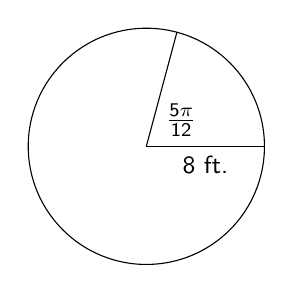
\begin{tikzpicture}[scale=0.75]
    \draw (0,0) circle [radius=2cm];
    \draw (0,0) -- node [midway, below] {\small 8 ft.} (2,0);
    \draw (0,0) -- (75:2);
    \node at (0,0) [above right, xshift=0.125cm] {$\tfrac{5\pi}{12}$};
    \end{tikzpicture}
    
    \item \mbox{} \newline\\
    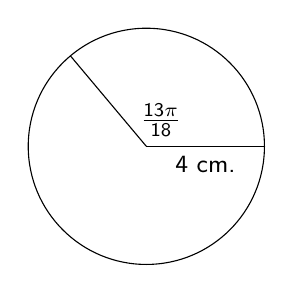
\begin{tikzpicture}[scale=0.75]
    \draw (0,0) circle [radius=2cm];
    \draw (0,0) -- node [midway, below] {\small 4 cm.} (2,0);
    \draw (0,0) -- (130:2);
    \node at (0,0) [above right, xshift=-0.2cm] {$\tfrac{13\pi}{18}$};
    \end{tikzpicture}
    
    \item \mbox{} \newline\\
    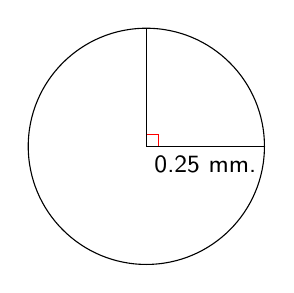
\begin{tikzpicture}[scale=0.75]
    \draw (0,0) circle [radius=2cm];
    \draw[red] (0,0) rectangle +(0.2,0.2);
    \draw (0,0) -- node [midway, below] {\small 0.25 mm.} (2,0);
    \draw (0,0) -- (90:2);
    \end{tikzpicture}
\end{enumerate}	\setcounter{Review}{\value{enumi}}
\end{multicols}

A belt runs on a pulley with radius 4 inches at 250 revolutions per minute.
\begin{enumerate} \setcounter{enumi}{\value{Review}}
\item Find the angular velocity in rad/sec. Round your answer to 2 decimal places.
    \item Find the linear velocity in ft/sec. Round your answer to 2 decimal places.
\end{enumerate}	\setcounter{Review}{\value{enumi}}

\newpage

\section{Answer Key}

\begin{enumerate}
	\item $\frac{5\pi}{4}$  \newline\\
    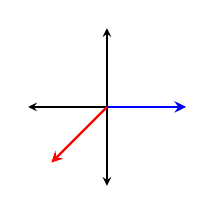
\begin{tikzpicture}
    \draw [<->, >=stealth](-1,0) -- (1,0);
    \draw[<->, >=stealth](0,-1) -- (0,1);
    \draw[->, thick, >=stealth, blue](0,0)--(1,0);
    \draw[->, thick, >=stealth, color=red](0,0) -- (-135:1);
    \bigangle[violet,thick]{-135}    
    \end{tikzpicture}
    
    \item $180^\circ$   \newline\\
    \begin{tikzpicture}
    \draw [<->, >=stealth](-1,0) -- (1,0);
    \draw[<->, >=stealth](0,-1) -- (0,1);
    \draw[->, thick, >=stealth, blue](0,0)--(1,0);
    \draw[->, thick, >=stealth, color=red](0,0) -- (180:1);
    \bigangle[violet,thick]{900}    
    \end{tikzpicture}
    
    \item $\frac{7\pi}{10}$ \newline\\
    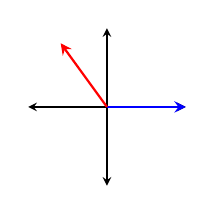
\begin{tikzpicture}
    \draw [<->, >=stealth](-1,0) -- (1,0);
    \draw[<->, >=stealth](0,-1) -- (0,1);
    \draw[->, thick, >=stealth, blue](0,0)--(1,0);
    \draw[->, thick, >=stealth, color=red](0,0) -- (486:1);
    \bigangle[violet,thick]{486}    
    \end{tikzpicture}
    
    \item $235^\circ$   \newline\\
    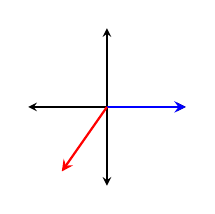
\begin{tikzpicture}
    \draw [<->, >=stealth](-1,0) -- (1,0);
    \draw[<->, >=stealth](0,-1) -- (0,1);
    \draw[->, thick, >=stealth, blue](0,0)--(1,0);
    \draw[->, thick, >=stealth, color=red](0,0) -- (-125:1);
    \bigangle[violet,thick]{-125}    
    \end{tikzpicture}
    
    \item $s = \frac{10\pi}{3}\,\mathrm{ft.}; \quad A = \frac{40\pi}{3}\,\mathrm{sq. ft.}$
    \item $s = \frac{26\pi}{9}\,\mathrm{cm.}; \quad A = \frac{52\pi}{9}\,\mathrm{sq. cm.}$
    \item $s = \frac{\pi}{8}\,\mathrm{mm.}; \quad A = \frac{\pi}{64}\,\mathrm{sq. mm.}$
    
    \item 26.18 rad/sec
    \item 8.73 ft/sec
\end{enumerate}
\chapter{Trig Functions of Any Angle}

Find the exact value of each of the six trig functions of $\theta$ if $P$ is a point on the terminal side of $\theta$.

\begin{enumerate}
	\item $P(-2, 3)$
	\item $P(0,-4)$
	\item $P(-2\sqrt{3}, 2)$
	\item $P(-3, 5)$
	\item $P(-2, 1)$
	\item $P(-4, -7)$
\end{enumerate}	\setcounter{Review}{\value{enumi}}

Find the exact values of the 6 trig functions of the following angles.

\begin{enumerate}		\setcounter{enumi}{\value{Review}}
	\item $\theta = \frac{-17\pi}{4}$
	\item $\theta = \frac{21\pi}{2}$
	\item $\theta = 24\pi$
\end{enumerate}

\newpage

\textsc{Trig Functions of Any Angle Key}

\begin{enumerate}
	\item $\sin\theta = \frac{3\sqrt{13}}{13}, \, \cos\theta = \frac{-2\sqrt{13}}{13}, \, \tan\theta = -\frac{3}{2}, \, \csc\theta = \frac{\sqrt{13}}{3}, \, \sec\theta = -\frac{\sqrt{13}}{2}, \, \cot\theta = -\frac{2}{3}$

    \item $\sin\theta = -1, \, \cos\theta = 0, \, \tan\theta = \text{undef.}, \, \csc\theta = -1, \, \sec\theta = \text{undef.}, \, \cot\theta = 0$
    
    \item $\sin\theta = \frac{1}{2}, \, \cos\theta = -\frac{\sqrt{3}}{2}, \, \tan\theta = -\frac{\sqrt{3}}{3}, \, \csc\theta = 2, \, \sec\theta = -\frac{2\sqrt{3}}{3}, \, \cot\theta = -\sqrt{3}$
    
    \item $\sin\theta = -\frac{\sqrt{2}}{2}, \quad \cos\theta = \frac{\sqrt{2}}{2}, \quad \tan\theta = -1, \quad \csc\theta = -\sqrt{2}, \quad \sec\theta = \sqrt{2}, \quad \cot\theta = -1$
    
    \item $\sin\theta = 1, \quad \cos\theta = 0, \quad \tan\theta = \text{undefined}, \quad \csc\theta = 1, \quad \sec\theta = \text{undefined}, \quad \cot\theta = 0$
    
    \item $\sin\theta = 0, \quad \cos\theta = 1, \quad \tan\theta = 0, \quad \csc\theta = \text{undefined}, \quad \sec\theta = 1, \quad \cot\theta = \text{undefined}$
    
    
\end{enumerate}
\chapter{Graphs of Sine and Cosine Functions}

Determine the amplitude, period, phase shift, and vertical shift for each. Exact answers only.

\begin{enumerate}
	\item $f(x) = -2\sin\left(3x-\frac{\pi}{4}\right) + 1$
	\item $g(x) = \frac{1}{3}\cos\left(\frac{1}{2}x + 2\right)$
	\item $f(x)=2\sin\left(x-\frac{\pi}{3}\right)+7$
	\item $f(x)=-4\cos\left(\frac{2}{3}x-\frac{2\pi}{3}\right)$
\end{enumerate}
\setcounter{Review}{\value{enumi}}

Write the equation of each of the following in the form $y = a\sin(bx)$.
\begin{multicols}{2}
\begin{enumerate}	\setcounter{enumi}{\value{Review}}
	\item \mbox{} \newline\\ 
	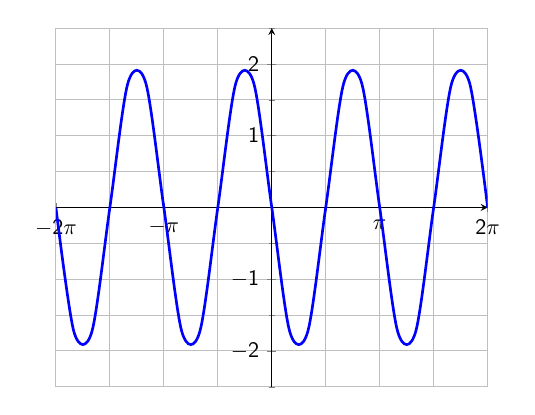
\begin{tikzpicture}[scale=0.8]
    \begin{axis}[
    axis lines = middle, xmin = -2*pi, xmax = 2*pi, ymin=-2.5, ymax=2.5, xtick={-2*pi, -pi, 0, pi, 2*pi}, xticklabels={$-2\pi$, $-\pi$, 0, $\pi$, $2\pi$}, grid=both, minor tick num = 1]
    \addplot[blue, very thick, domain=-2*pi:2*pi, smooth] {-2*sin(2*deg(x))};
    \end{axis}
    \end{tikzpicture}
    
    \item \mbox{} \newline\\
    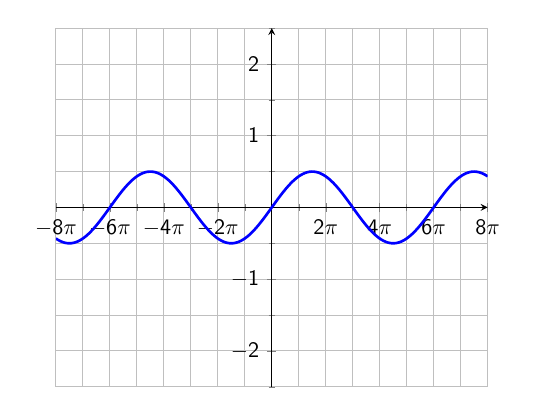
\begin{tikzpicture}[scale=0.8]
    \begin{axis}[
    axis lines = middle, xmin = -8*pi, xmax = 8*pi, ymin=-2.5, ymax=2.5, xtick={-8*pi,-6*pi,-4*pi,-2*pi, 0, 2*pi, 4*pi, 6*pi, 8*pi}, xticklabels={$-8\pi$, $-6\pi$, $-4\pi$, $-2\pi$, 0, $2\pi$, $4\pi$, $6\pi$, $8\pi$}, grid=both, minor tick num = 1]
    \addplot[blue, very thick, domain=-8*pi:8*pi, samples=200] {(1/2)*sin((1/3)*deg(x))};
    \end{axis}
    \end{tikzpicture}
\end{enumerate}
\end{multicols}

\newpage

\textsc{Answers}

\begin{enumerate}
	\item Amp = 2, Per = $\frac{2\pi}{3}$, P.S. = $\frac{\pi}{12} \rightarrow$, V.S. = $1 \uparrow$
    \item Amp = $\frac{1}{3}$, Per = $4\pi$, P.S. = $4 \leftarrow$, V.S. = None
    \item Amp = 2, Period = $2\pi$, P.S. = $\frac{\pi}{3}$ right, V.S. = 7 up
    \item Amp = 4, Period = $3\pi$, P.S. = $\pi$ right, V.S. = 0 (or none)
    
    \item $y = -2\sin(2x)$
	\item $y = \frac{1}{2}\sin\left(\frac{1}{3}x\right)$
\end{enumerate}
\chapter{Graphs of Other Trig Functions}

Determine the amplitude, period, phase shift, and vertical shift for each. Exact answers only.

\begin{enumerate}
	\item $h(x) = \tan\left(\frac{3}{4}x + \frac{\pi}{12}\right) - 8$
	\item $f(x)=3\tan\left(-2x+\frac{\pi}{2}\right)-\sqrt{3}$
\end{enumerate}

\newpage

\textsc{Graphs of Other Trig Functions Key}

\begin{enumerate}
	\item Amp = n/a, Per = $\frac{4\pi}{3}$, P.S. = $\frac{\pi}{9} \leftarrow$, V.S. = $8 \downarrow$
\end{enumerate}
\chapter{Inverse Trig Functions}

State the exact, simplified value of each or write as an expression of $x$.

\begin{multicols}{3}
\begin{enumerate}
	\item $\cot^{-1}\left(-1\right)$
	\item $\sin^{-1}\left(-\frac{\sqrt{3}}{2	}\right)$
	\item $\tan^{-1}\left(0\right)$
\end{enumerate}	\setcounter{Review}{\value{enumi}}
\end{multicols}
\smallskip
\begin{multicols}{3}
\begin{enumerate}	\setcounter{enumi}{\value{Review}}
	\item $\sec^{-1}\left(\frac{2\sqrt{3}}{3}\right)$
	\item $\cos^{-1}\left(\frac{1}{2}\right)$
	\item $\sec^{-1}\left(-2\right)$
\end{enumerate}	\setcounter{Review}{\value{enumi}}
\end{multicols}
\smallskip
\begin{multicols}{3}
\begin{enumerate}	\setcounter{enumi}{\value{Review}}
	\item $\tan^{-1}\left(-\sqrt{3}\right)$
	\item $\sec\left(\sin^{-1}\left(\frac{2}{5}\right)\right)$
	\item $\cot\left(\sec^{-1}(x)\right)$
\end{enumerate}	\setcounter{Review}{\value{enumi}}
\end{multicols}
\smallskip
\begin{multicols}{3}
\begin{enumerate}	\setcounter{enumi}{\value{Review}}
	\item $\sin\left(\cos^{-1}\left(\frac{3x}{4}\right)\right)$
	\item $\cot\left(\csc^{-1}\left(-\frac{7}{2}\right)\right)$
	\item $\sec\left(\arcsin\left(\frac{9}{13}\right)\right)$
\end{enumerate}	\setcounter{Review}{\value{enumi}}
\end{multicols}
\smallskip
\begin{multicols}{3}
\begin{enumerate}	\setcounter{enumi}{\value{Review}}
	\item $\cos\left(\tan^{-1}(7x)\right)$
	\item $\sin\left(\sec^{-1}\left(\frac{8}{x}\right)\right)$
	\item $\csc\left(\arctan\left(-\frac{3}{2}\right)\right)$
\end{enumerate}	\setcounter{Review}{\value{enumi}}
\end{multicols}
\smallskip
\begin{multicols}{3}
\begin{enumerate}	\setcounter{enumi}{\value{Review}}
	\item $\cos\left(\sin^{-1}\left(\frac{7}{8}\right)\right)$
	\item $\tan\left(\cos^{-1}\left(\frac{3}{x}\right)\right)$
	\item $\csc\left(\sec^{-1}\left(\sqrt{2}\right)\right)$
\end{enumerate}	\setcounter{Review}{\value{enumi}}
\end{multicols}
\smallskip
\begin{multicols}{3}
\begin{enumerate}	\setcounter{enumi}{\value{Review}}
	\item $\tan\left(\sec^{-1}\left(\frac{\sqrt{17}}{4}\right)\right)$
	\item $\sin\left(\tan^{-1}\left(\frac{4x}{5}\right)\right)$
	\item $\cos\left(\tan^{-1}\left(\frac{\sqrt{3}}{5}\right)\right)$
\end{enumerate}	\setcounter{Review}{\value{enumi}}
\end{multicols}
\smallskip
\begin{multicols}{3}
\begin{enumerate}	\setcounter{enumi}{\value{Review}}
	\item $\sin\left(\cos^{-1}\left(\frac{9}{10}\right)\right)$
	\item $\tan\left(\cot^{-1}\left(8\right)\right)$
\end{enumerate}	\setcounter{Review}{\value{enumi}}
\end{multicols}
\smallskip
\newpage

\section{Answer Key}

\begin{enumerate}
	\item $\frac{3\pi}{4}$
	\item $-\frac{\pi}{3}$
	\item 0
	\item $\frac{\pi}{6}$
	\item $\frac{\pi}{3}$
	\item $\frac{2\pi}{3}$
	\item $-\frac{\pi}{3}$
    \item $\frac{5\sqrt{21}}{21}$
    \item $\frac{1}{\sqrt{x^2-1}} = \frac{\sqrt{x^2-1}}{x^2-1}$
    \item $\frac{\sqrt{16-9x^2}}{4}$
    \item $-\frac{3\sqrt{5}}{2}$
    \item $\frac{13\sqrt{22}}{44}$
    \item $\frac{\sqrt{49x^2+1}}{49x^2+1}$
    \item $\frac{\sqrt{64-x^2}}{x}$
    \item $-\frac{\sqrt{13}}{3}$
    \item $\frac{\sqrt{15}}{8}$
    \item $\frac{\sqrt{x^2-9}}{3}$
    \item $\sqrt{2}$
    \item $\sqrt{17}$
    \item $\frac{4x}{\sqrt{16x^2+25}}$
    \item $\frac{5\sqrt{7}}{14}$
    \item $\frac{\sqrt{19}}{10}$
    \item $\frac{1}{8}$
\end{enumerate}

\chapter{Trig Equations and Inequalities}

Solve each in the interval $[0,2\pi)$. Write your answers to inequalities using interval notation.

\begin{enumerate}
	\item $\tan(6x) = 1$
    \item $\cot(2x) = -\frac{\sqrt{3}}{3}$
    \item $\sin^2 (x) = \frac{3}{4}$
    \item $\sin(2x) = \cos(x)$
    \item $\sin(2x) \geq \sin(x)$
    \item $\cos(2x) < 0$
    \item $2\sin\left(x-\frac{\pi}{3}\right) = -1$
    \item $3\tan\left(-2x+\frac{\pi}{2}\right)=\sqrt{3}$
    \item $\sin^2(x) < \frac{1}{2}$
    
    \item $\tan^2(x) = 3\sec(x) - 3$
    \item $2\csc(x) - 3\csc^2(x) = -2\csc^2(x) + 1$
    \item $-2\cot(x) - \csc^2(x) = 0$
    \item $\tan(x) = -\tan(x)\cos(x)$
    \item $3\cos(x) = 2\cos^2(x) + 1$
    \item $\csc(x) - \cot^2(x) + 1 = 0$
    \item $-\sin(x) + \sin(2x) = 2\sin(2x)$
    \item $3\cos(x) = \sin(2x) + 2\cos(x)$
\end{enumerate}

\newpage

\section{Answer Key}

\begin{enumerate}
	\item $\frac{\pi}{24}, \frac{5\pi}{24}, \frac{3\pi}{8}, \frac{13\pi}{24}, \frac{17\pi}{24}, \frac{7\pi}{8}, \frac{25\pi}{24}, \frac{29\pi}{24}, \frac{11\pi}{8}, \frac{37\pi}{24}, \frac{41\pi}{24}, \frac{15\pi}{8}$
    
	\item $\frac{\pi}{3}, \frac{5\pi}{6}, \frac{4\pi}{3}, \frac{11\pi}{6}$
    
	\item $\frac{\pi}{3}, \frac{2\pi}{3}, \frac{4\pi}{3}, \frac{5\pi}{3}$
    
	\item $\frac{\pi}{2}, \frac{5\pi}{6}, \frac{3\pi}{2}$
    
	\item $\left[0, \frac{\pi}{3}\right] \cup \left[\pi, \frac{5\pi}{3}\right]$
    
	\item $\left(\frac{\pi}{4}, \frac{3\pi}{4}\right) \cup \left(\frac{5\pi}{4}, \frac{7\pi}{4}\right)$
	
	\item $x = \frac{\pi}{6}, \, \frac{3\pi}{2}$
	
	\item $x = \frac{\pi}{6}, \, \frac{2\pi}{3}, \, \frac{7\pi}{6}, \, \frac{5\pi}{3}$
	
    \item $\left[0, \frac{\pi}{4}\right) \cup \left(\frac{3\pi}{4}, \frac{5\pi}{4}\right) \cup \left(\frac{7\pi}{4}, 2\pi\right)$
    
    \item $x = 0 \, \frac{\pi}{3}, \, \frac{5\pi}{3}$
    
    \item $x = \frac{\pi}{2}$
    
    \item $x = \frac{3\pi}{4}, \, \frac{7\pi}{4}$
    \item $x = 0, \, \pi$
    \item $x = 0 \, \frac{\pi}{3}, \, \frac{5\pi}{3}$
    \item $x = \frac{\pi}{6}, \, \frac{5\pi}{6}, \, \frac{3\pi}{2}$
    \item $x = 0, \, \frac{2\pi}{3}, \, \pi, \, \frac{4\pi}{3}$
    \item $x = \frac{\pi}{6}, \, \frac{\pi}{2}, \, \frac{5\pi}{6}, \, \frac{3\pi}{2}$
\end{enumerate}
\chapter{Law of Sines and Cosines}

Solve each of the following. Round your answers to 1 decimal place.

\begin{enumerate}
	\item $m\angle B = 37.8^\circ, \, a = 15, \, c = 21.1$
    \item $m\angle A = 41.9^\circ, \, m\angle C = 59.2^\circ, \, a = 10.2$
    \item $a = 14, \, b = 19.6, \, c = 13.1$
\end{enumerate}

\newpage

\textsc{Law of Sines and Cosines Key}

\begin{enumerate}
	\item $b \approx 13.0, \, m\angle A \approx 44.8^\circ, \, m\angle C \approx 97.4^\circ$
	\item $m \angle B = 78.9^\circ, \, b \approx 15.0, \, c \approx 13.1$
	\item $m\angle A \approx 45.5^\circ, \, m\angle B \approx 92.6^\circ, \, m\angle C \approx 41.9^\circ$
\end{enumerate}
\chapter{Area of Triangles}

Find the area of each. Round your answers to 1 decimal place.

\begin{enumerate}
	\item $m\angle B = 37.8^\circ, \, a = 15, \, c = 21.1$
    \item $m\angle A = 41.9^\circ, \, m\angle C = 59.2^\circ, \, a = 10.2$
    \item $a = 14, \, b = 19.6, \, c = 13.1$
    
    \item $p = 14, \, k = 9, \, h = 9$
    \item $m\angle T = 15^\circ, \, m\angle S = 140^\circ, \, r = 11.1$
    \item $m\angle Z = 67^\circ, \, y = 6, \, m\angle Y = 41^\circ$
    \item $m\angle R = 129^\circ, \, r = 10, \, m\angle P = 28^\circ$
    \item $a = 6.9, \, m\angle B = 115^\circ, m\angle C = 39^\circ$
    \item $d = 6, \, 3 = 12, \, f = 8$
    \item $m\angle Y = 120^\circ, \, x = 13, \, m\angle Z = 21^\circ$
    \item $z = 10, \, y = 14, \, x = 6$
    \item $m\angle P = 18^\circ, \, h = 6.9, \, m\angle H = 147^\circ$
    \item $m\angle S = 118^\circ, \, m\angle T = 30^\circ, \, s = 6.3$
    \item $r = 8, \, t = 7.5, \, m\angle S = 50^\circ$
    \item $d = 15.3, \, m\angle E = 105^\circ, \, f = 5$
    \item $m\angle R = 31^\circ, \, p = 12, \, m\angle Q = 26^\circ$
    \item $m\angle D = 120^\circ, \, f = 4, \, m\angle E = 36^\circ$
\end{enumerate}

\newpage

\section{Answer Key}

\begin{enumerate}
	\item Approximately 97.0 sq. units
	\item Approximately 65.7 sq. units
	\item Approximately 91.6 sq. units
	\item Approximately 39.6 sq. units
	\item Approximately 24.3 sq. units
	\item Approximately 24.0 sq. units
	\item Approximately 11.7 sq. units
	\item Approximately 31.0 sq. units
	\item Approximately 21.3 sq. units
	\item Approximately 41.7 sq. units
	\item Approximately 26.0 sq. units
	\item Approximately 3.5 sq. units
	\item Approximately 6.0 sq. units
	\item Approximately 23.0 sq. units
	\item Approximately 36.9 sq. units
	\item Approximately 19.5 sq. units
	\item Approximately 10.0 sq. units
\end{enumerate}
\appendix
\chapter{Factoring}

Factor each of the following completely.

\begin{multicols}{4}
\begin{enumerate}
\item $x^2 + 2x - 15$
\item $x^2 - 8x + 12$
\item $x^2 + 15x + 56$
\item $5x^2 + 19x - 4$
\item $4x^2 - 5x - 6$
\item $9x^2 - 400$
\item $5x^2-7x-6$
\item $9x^2-54x+45$
\item $3x^3+12x^2+9x$
\item $9y^2-16$
\item $4x^2-28x+49$
\item $14x^2+11xy-15y^2$
\item $6x^2-48x-120$
\item $9x^4-54x^3+45x^2$
\item $16y^2-40y+25$
\item $30x^2+xy-y^2$
\item $8w^2 + 33w + 4$
\item $3p^2+22p-16$
\item $18x^2-27x+4$
\item $14a^2+15a-9$
\item $4x^2-4x-24$
\item $18t^2-9t-5$
\item $6a^2 + 23a + 21$
\item $25x^2-1$
\end{enumerate}
\end{multicols}

\newpage

\section{Answer Key}

\begin{multicols}{4}
\begin{enumerate}
\item $(x + 5)(x-3)$
\item $(x-6)(x-2)$
\item $(x+7)(x+8)$
\item $(5x-1)(x+4)$
\item $(4x+3)(x-2)$
\item $(3x+20)(3x-20)$
\item $(5x+3)(x-2)$
\item $9(x-5)(x-1)$
\item $3x(x+3)(x+1)$
\item $(3y+4)(3y-4)$
\item $(2x-7)^2$
\item $(7x - 5y)(2x + 3y)$
\item $6(x-10)(x+2)$
\item $9x^2(x-1)(x-5)$
\item $(4y-5)^2$
\item $(6x-y)(5x+y)$
\item $(8w+1)(w+4)$
\item $(3p-2)(p+8)$
\item $(6x-1)(3x-4)$
\item $(7a-3)(2a+3)$
\item $4(x-3)(x+2)$
\item $(6t-5)(3t+1)$
\item $(2a+3)(3a+7)$
\item $(5x+1)(5x-1)$
\end{enumerate}
\end{multicols}
\chapter{Complex Fractions}

Simplify each as much as possible.

\begin{multicols}{3}
\begin{enumerate}
\setlength\itemsep{10pt}
\item $\frac{5+\frac{3}{x}}{x-\frac{1}{2}}$
\item $\frac{\frac{1}{x}+\frac{2}{x^2}}{x+\frac{8}{x^2}}$
\item $\frac{3}{2-\frac{x}{x-1}}$
\item $\frac{1+\frac{3}{x}}{\frac{2}{x}+7}$
\item $\frac{\frac{4}{x}-\frac{x}{x-2}}{\frac{1}{x}+{\frac{3}{x-2}}}$
\item $\frac{\frac{3}{x+1}-4}{\frac{2}{x+1}}$
\item $\frac{\frac{5}{x}+\frac{3}{x-2}}{\frac{7}{x^2-2x}}$
\item $\frac{\frac{1}{x}-\frac{1}{7}}{x-7}$
\item $\frac{\frac{1}{x}+\frac{1}{x+1}}{5}$
\item $\frac{\frac{5}{x}-5x}{x-1}$
\item $\frac{\frac{1}{2+x}-\frac{1}{2}}{x}$
\item $\frac{\frac{3}{x-4}+\frac{2x}{x+1}}{4x}$
\item $\frac{\frac{1}{x-a}+\frac{1}{a}}{x}$
\item $\dfrac{\frac{1}{x-1}-\frac{1}{x-3}}{\frac{2}{x-1}+\frac{3}{x+1}}$
\item $\dfrac{\frac{2}{x^2-4}+\frac{1}{x-2}}{\frac{4}{x+2}}$
\end{enumerate}
\end{multicols}

\newpage

\section{Answer Key}

\begin{multicols}{3}
\begin{enumerate}
\setlength\itemsep{10pt}
\item $\frac{2(5x+3)}{x(2x-1)}$
\item $\frac{1}{x^2-2x+4}$
\item $\frac{3(x-1)}{x-2}$
\item $\frac{x+3}{2+7x}$
\item $\frac{-1(x^2-4x+8)}{2(2x-1)}$
\item $\frac{-4x-1}{2}$
\item $\frac{8x-10}{7}$
\item $-\frac{1}{7x}$
\item $\frac{2x+1}{5x(x+1)}$
\item $\frac{-5x-5}{x}$
\item $\frac{-1}{2x+4}$
\item $\frac{(x-1)(2x-3)}{4x(x-4)(x+1)}$
\item $\frac{1}{a(x-a)}$
\item $\frac{-2x-2}{5x^2-16x+3}$
\item $\frac{x+4}{4x-8}$
\end{enumerate}
\end{multicols}
\end{document}